\section{F�nix Firewall System}

\begin{frame}
  \frametitle{Conhecendo a F�nix}
  
			\begin{figure}[htbp]
				\centering
					
\includegraphics[width=0.40\textwidth]{../Pictures/Baixa/Fenix_Picture.png}				
				\label{fig:Fenix_Picture}
			\end{figure}

\end{frame}

\begin{frame}
\frametitle{\alert{Pr�ximos Slides}}
			
			\begin{center}
					\huge \textbf{Vis�o Geral da Arquitetura}.
			\end{center}
			
\end{frame}

%_______________________________________________________________________
\subsection{Vis�o Geral da Arquitetura}

\begin{frame}
  \frametitle{Vis�o Geral da Arquitetura}
  \framesubtitle{Do que o F�nix � capaz?}

			\begin{itemize}
				\item \alert{Controlar} o acesso ao dispositivo.
				\item \alert{Restringir} acessos entrantes e/ou saintes:
				
						\begin{enumerate}
							\item Dom�nios (Ex.: www.hackers.org);
							\item Redes  (Ex.: 10.0.0.0/8);	
							\item Sub-redes (Ex.: 200.137.197.129/27);
							\item Faixa de Endere�os IP (Ex.: 172.13.0.1 - 172.13.0.10);
							\item Endere�o IP (Ex.: 192.168.1.1/24)
						\end{enumerate}
						
				\item \alert{Notificar} quando conex�es suspeitas surgirem.
				\item \alert{Carregar} pol�ticas de seguran�a e prefer�ncias de usu�rio segundo a \textbf{localiza��o}.
				\item \alert{Sincronizar} e receber \alert{notifica��es} de seguran�a com uma Plataforma Distribu�da (\textbf{Opcional}).
			\end{itemize}

\end{frame}

\begin{frame}
	\frametitle{Ataques detectados pelo F�nix}
  
			\begin{itemize}
				\item Varreduras de portas.
				\item Worms e Cavalos de Tr�ia.
				\item Ataques DoS (tradicionais).
				\item IP Spoofing.
				\item Roteamento dirigido.
				\item Ping O'Death.
				\item SYN Flood.
				\item Ataques contra o protocolo NETBIOS.
				\item Ataques contra o X-Windows.				
				\item Ataque de Fragmenta��o.
				\item Varredura invis�vel.
				\item Transpar�ncia dos dados na rede.				
			\end{itemize}

\end{frame}



\begin{frame}
  \frametitle{Vis�o Geral da Arquitetura}

		\begin{block}{Arquitetura do F�nix Firewall}		
			\begin{enumerate}
				\item \alert{\textbf{Arquitetura Embarcada}}.\\
							Instalada no Dispositivo M�vel.
											
				\item \alert{\textbf{Arquitetura Distribu�da}}.\\
							Parte \textbf{Opcional}, que � instalada em computadores na WEB. Interessante para \textbf{Usu�rios Avan�ados} e \textbf{Terceiros}.
							
			\end{enumerate}
		\end{block}

\end{frame}


%_______________________________________________________________________

\subsection{Arquitetura Embarcada}

\begin{frame}
  \frametitle{\alert{Pr�ximos Slides}}
			
			\begin{center}
					\huge \textbf{Arquitetura Embarcada}.
			\end{center}
			
\end{frame}


\begin{frame}
  \frametitle{Arquitetura Embarcada}
  
\begin{figure}[htbp]
	\centering
		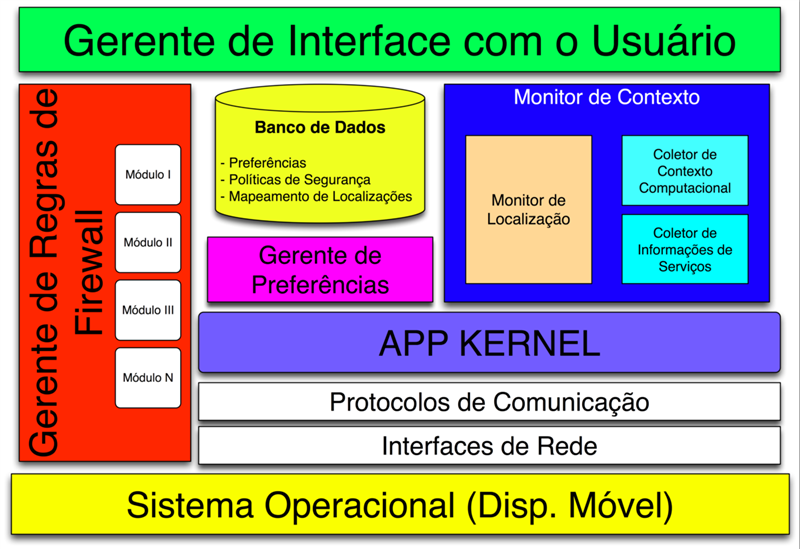
\includegraphics[width=0.80\textwidth]{../Pictures/Sequencias/Arquitetura_Embarcada/Arquitetura_Embarcada.png}
	\label{fig:Arquitetura_Embarcada}
\end{figure}
  
\end{frame}


\begin{frame}
  \frametitle{Arquitetura Embarcada}
  \framesubtitle{Sistema Operacional}
  
\begin{figure}[htbp]
	\centering
		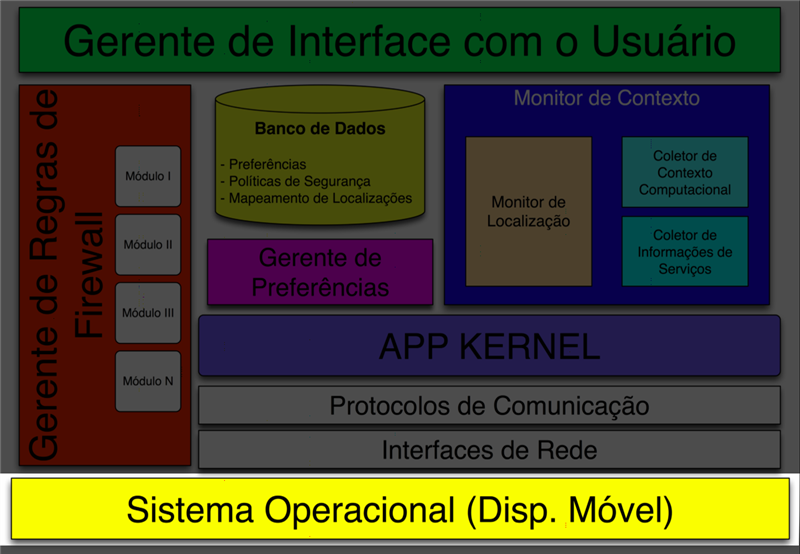
\includegraphics[width=0.80\textwidth]{../Pictures/Sequencias/Arquitetura_Embarcada/SistemaOperacional.png}
	\label{fig:SistemaOperacional}
\end{figure}
  
\end{frame}


\begin{frame}
  \frametitle{Arquitetura Embarcada}
  \framesubtitle{AppKernel \alert{(N�cleo)}}
  
\begin{figure}[htbp]
	\centering
		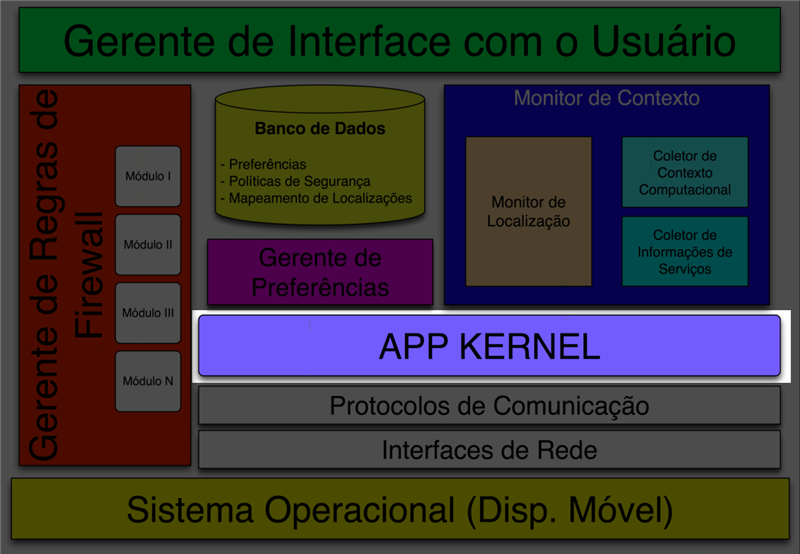
\includegraphics[width=0.80\textwidth]{../Pictures/Sequencias/Arquitetura_Embarcada/AppKernel.png}
	\label{fig:AppKernel}
\end{figure}
  
\end{frame}

\begin{frame}
  \frametitle{Arquitetura Embarcada}
  \framesubtitle{Gerente de Prefer�ncias}
  
\begin{figure}[htbp]
	\centering
		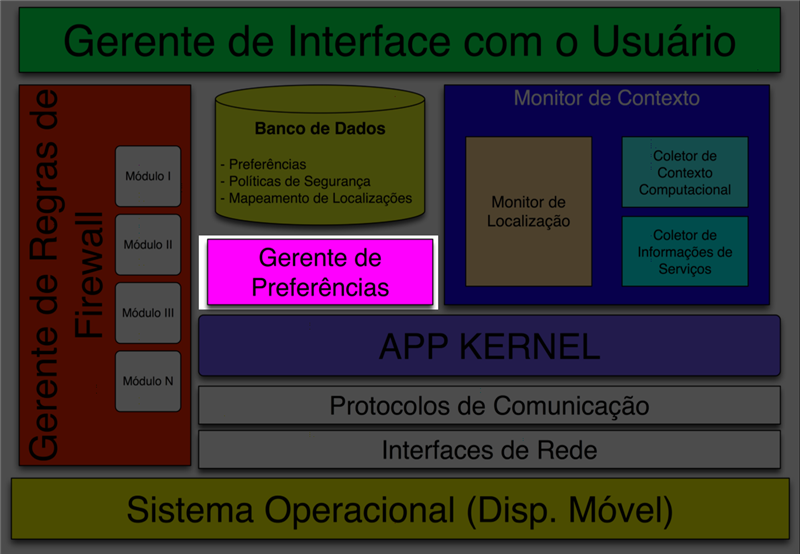
\includegraphics[width=0.80\textwidth]{../Pictures/Sequencias/Arquitetura_Embarcada/GerentePreferencias.png}
	\label{fig:GerentePreferencias}
\end{figure}
  
\end{frame}


\begin{frame}
  \frametitle{Arquitetura Embarcada}
	\framesubtitle{Banco de Dados}  
	
\begin{figure}[htbp]
	\centering
		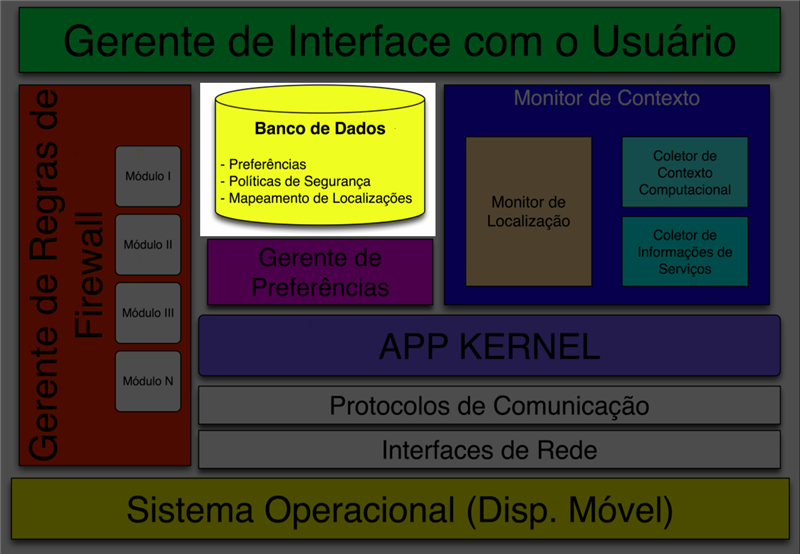
\includegraphics[width=0.80\textwidth]{../Pictures/Sequencias/Arquitetura_Embarcada/BancoDados.png}
	\label{fig:BancoDados}
\end{figure}
  
\end{frame}


\begin{frame}
  \frametitle{Arquitetura Embarcada}
  \framesubtitle{Gerente de Regras de Firewall}
  
\begin{figure}[htbp]
	\centering
		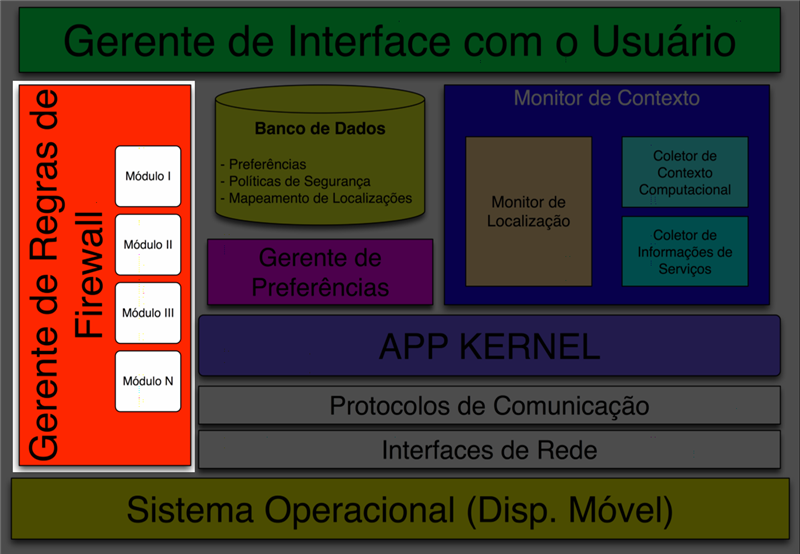
\includegraphics[width=0.80\textwidth]{../Pictures/Sequencias/Arquitetura_Embarcada/GerenteRegrasFirewall.png}
	\label{fig:GerenteRegrasFirewall}
\end{figure}
  
\end{frame}


\begin{frame}
  \frametitle{Arquitetura Embarcada}
  \framesubtitle{Monitor de Contexto}
  
\begin{figure}[htbp]
	\centering
		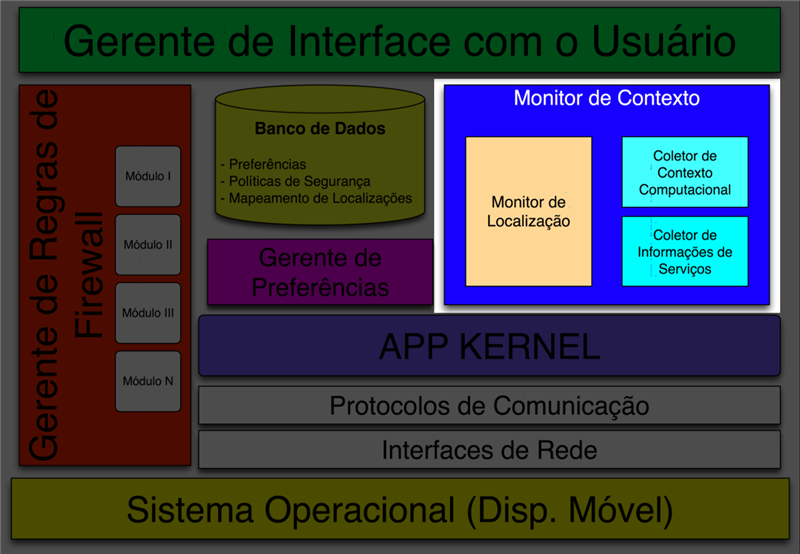
\includegraphics[width=0.80\textwidth]{../Pictures/Sequencias/Arquitetura_Embarcada/MonitorContexto.png}
	\label{fig:MonitorContexto}
\end{figure}
  
\end{frame}


\begin{frame}
  \frametitle{Arquitetura Embarcada}
  \framesubtitle{Monitor de Localiza��o}
  
\begin{figure}[htbp]
	\centering
		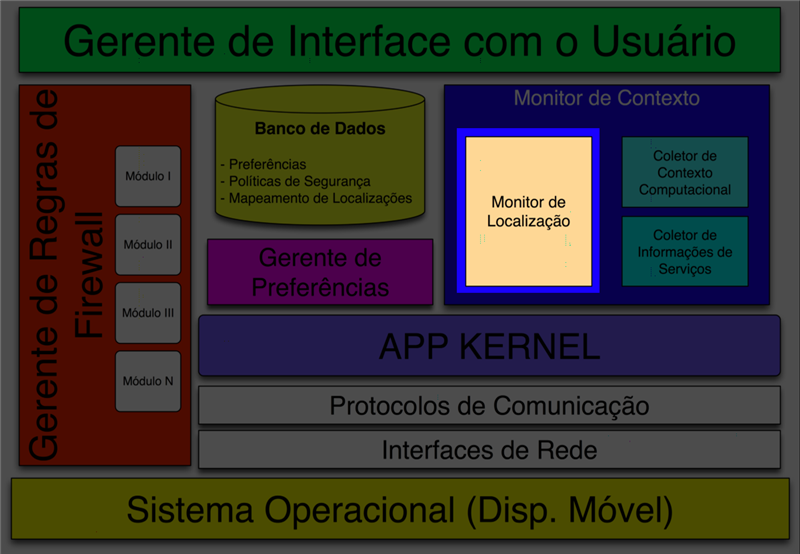
\includegraphics[width=0.80\textwidth]{../Pictures/Sequencias/Arquitetura_Embarcada/MonitorLocalizacao.png}
	\label{fig:MonitorLocalizacao}
\end{figure}
  
\end{frame}


\begin{frame}
  \frametitle{Arquitetura Embarcada}
  \framesubtitle{Coletor de Contexto Computacional}
  
\begin{figure}[htbp]
	\centering
		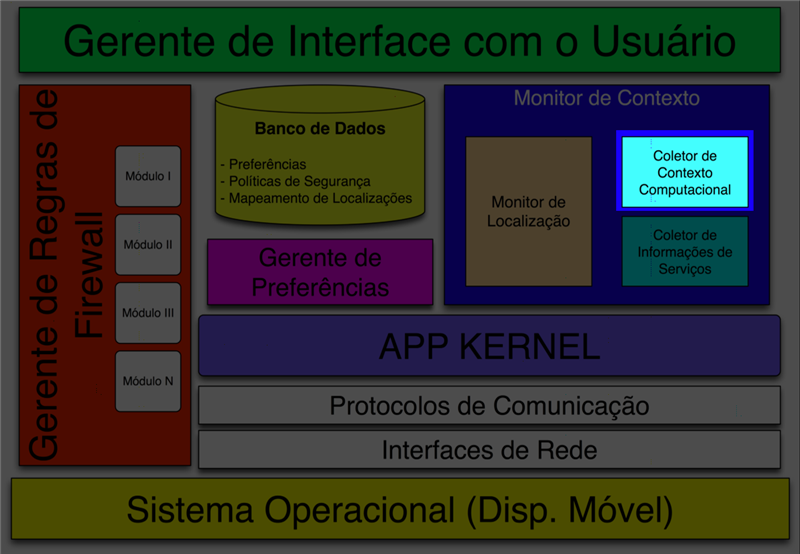
\includegraphics[width=0.80\textwidth]{../Pictures/Sequencias/Arquitetura_Embarcada/ColetorContextoComputacional.png}
	\label{fig:ColetorContextoComputacional}
\end{figure}
  
\end{frame}


\begin{frame}
  \frametitle{Arquitetura Embarcada}
  \framesubtitle{Coletor de Informa��es de Servi�os}
  
\begin{figure}[htbp]
	\centering
		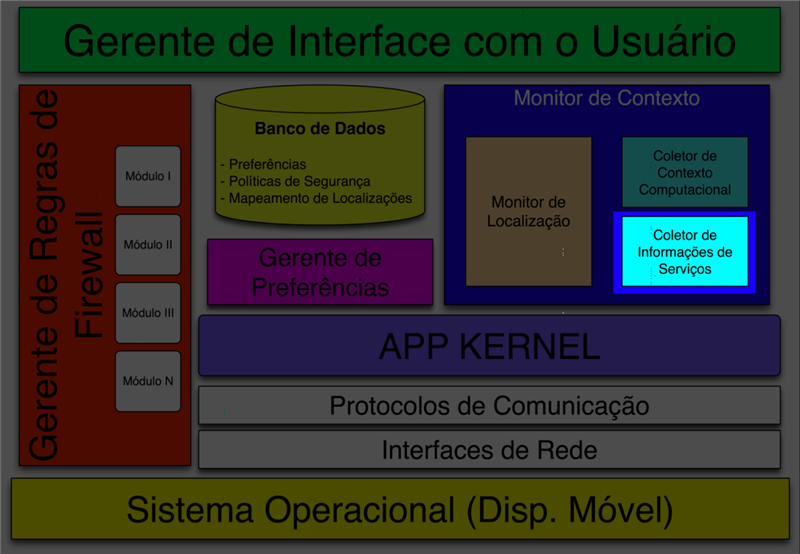
\includegraphics[width=0.80\textwidth]{../Pictures/Sequencias/Arquitetura_Embarcada/ColetorInformacoesServico.png}
	\label{fig:ColetorInformacoesServico}
\end{figure}
  
\end{frame}


\begin{frame}
  \frametitle{Arquitetura Embarcada}
  \framesubtitle{Gerente de Interfaces}
  
\begin{figure}[htbp]
	\centering
		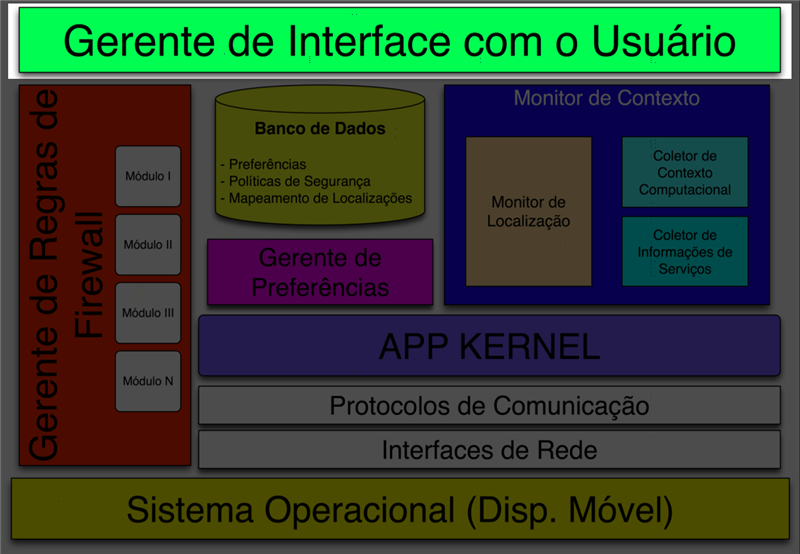
\includegraphics[width=0.80\textwidth]{../Pictures/Sequencias/Arquitetura_Embarcada/GerenteInterface.png}
	\label{fig:GerenteInterface}
\end{figure}
  
\end{frame}


\begin{frame}
  \frametitle{Arquitetura Embarcada}
  
\begin{figure}[htbp]
	\centering
		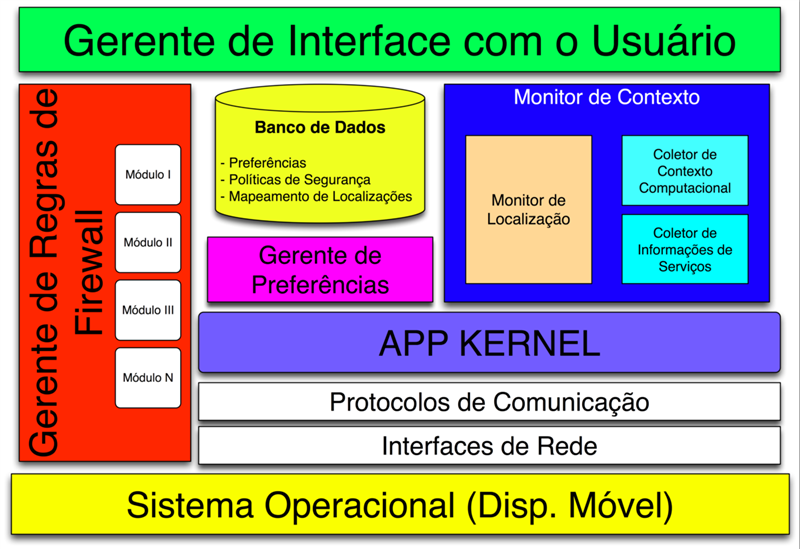
\includegraphics[width=0.80\textwidth]{../Pictures/Sequencias/Arquitetura_Embarcada/Arquitetura_Embarcada.png}
	\label{fig:Arquitetura_Embarcada}
\end{figure}
  
\end{frame}





%_______________________________________________________________________

\subsection{Arquitetura Distribu�da}

\begin{frame}
  \frametitle{\alert{Pr�ximos Slides}}
			
			\begin{center}
					\huge \textbf{Arquitetura Distribu�da}.
			\end{center}
			
\end{frame}

\begin{frame}
  \frametitle{Arquitetura Distribu�da}
  \framesubtitle{Vis�o Geral}
  
			\begin{figure}[htbp]
				\centering 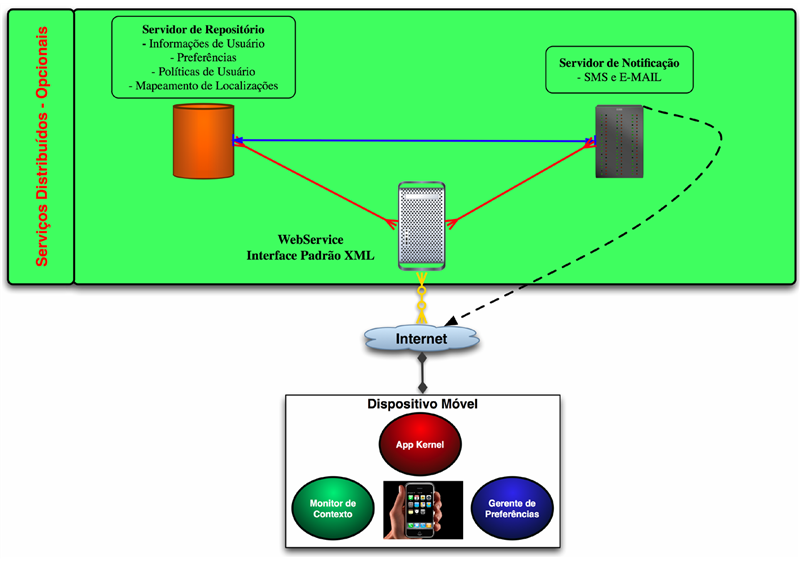
\includegraphics[width=0.80\textwidth]{../Pictures/Sequencias/Arquitetura_Distribuida/Arquitetura_Distribuida.png}
				\label{fig:Arquitetura_Distribuida}
			\end{figure}

\end{frame}


\begin{frame}[allowframebreaks]
		\frametitle{Plataforma Distribu�da (Uma \alert{\textbf{Op��o}} Inteligente)}
		
		
		\begin{block}{Controle de acesso gerenciado por grupos}
				\begin{enumerate}
						\item \alert{\textbf{Administradores}}
						\\ Grupo de usu�rios com acesso privilegiado respons�vel pela ger�ncia e manuten��o da plataforma distribu�da.
						\item \alert{\textbf{Usu�rios}}
						\\ Grupo de usu�rios ordin�rios com acesso restrito � plataforma distribu�da.
				\end{enumerate}			
		\end{block}
		
		\newpage		
		\begin{itemize}
			\item Facilita \alert{ger�ncia} dos dispositivos m�veis por \textbf{terceiros}.
			\item Permite maior \alert{integra��o} entre os dispositivos m�veis.
			\item Permite que o \alert{Administrador} envie notifica��es importantes aos usu�rios.
			\item Permite que o \alert{Administrador} insira uma nova pol�tica de seguran�a de forma autorit�ria, evitando ataques do tipo \textbf{0-day (Zero Day)}.								
			\item Permite que o usu�rio \textbf{troque de dispositivo} e mantenha as mesmas prefer�ncias e pol�ticas de seguran�a.			
		\end{itemize}
		
\end{frame}


\begin{frame}
  \frametitle{Arquitetura Distribu�da}
  \framesubtitle{Dispositivo M�vel}
  
\begin{figure}[htbp]
	\centering
		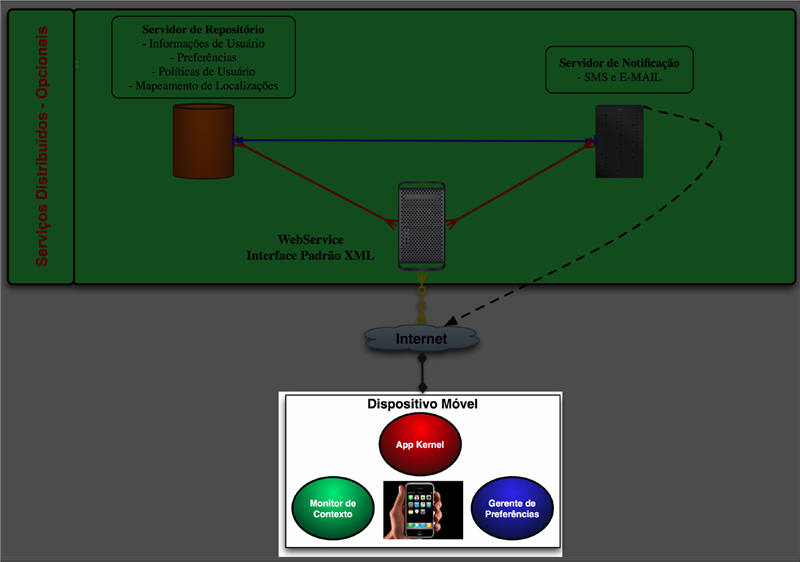
\includegraphics[width=0.80\textwidth]{../Pictures/Sequencias/Arquitetura_Distribuida/DispositivoMovel.png}
	\label{fig:DispositivoMovel}
\end{figure}

\end{frame}


\begin{frame}
  \frametitle{Arquitetura Distribu�da}
  \framesubtitle{Conex�o com a Internet}
  
\begin{figure}[htbp]
	\centering
		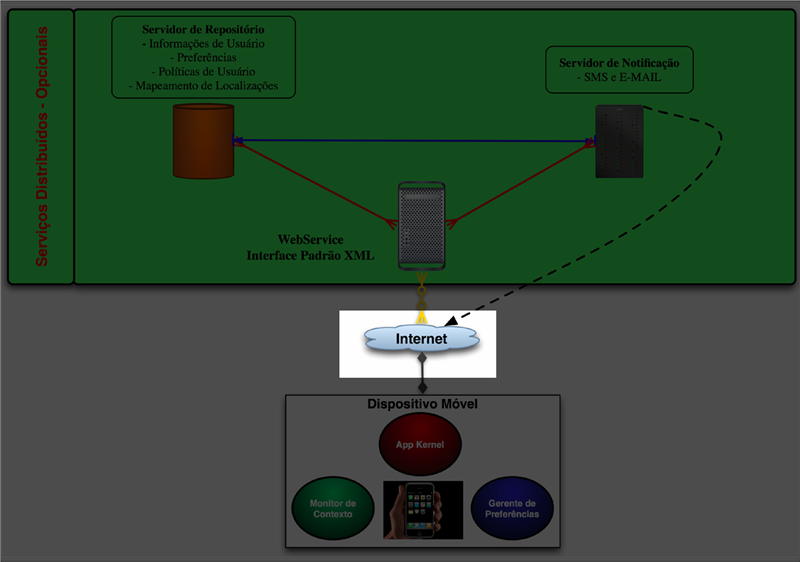
\includegraphics[width=0.80\textwidth]{../Pictures/Sequencias/Arquitetura_Distribuida/Internet.png}
	\label{fig:Internet}
\end{figure}

\end{frame}


\begin{frame}
  \frametitle{Arquitetura Distribu�da}
  \framesubtitle{Servidor WebService}
  
\begin{figure}[htbp]
	\centering
		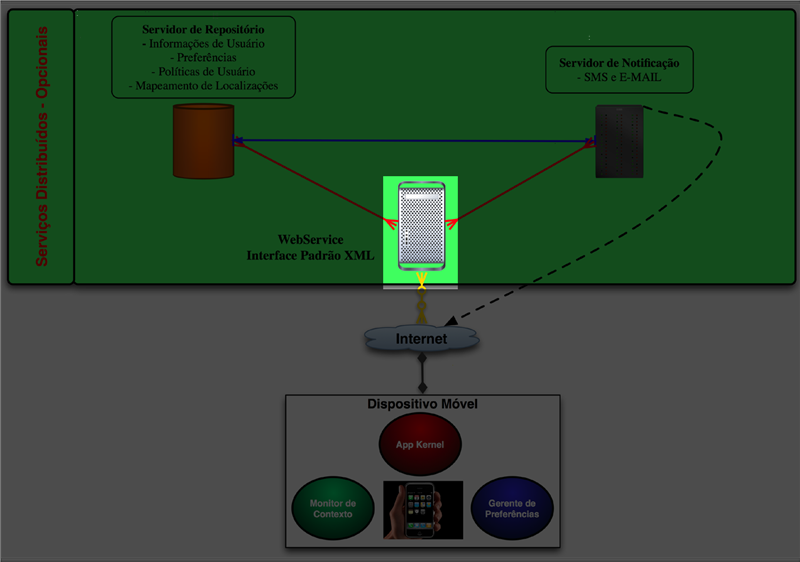
\includegraphics[width=0.80\textwidth]{../Pictures/Sequencias/Arquitetura_Distribuida/WebService.png}
	\label{fig:WebService}
\end{figure}

\end{frame}

\begin{frame}
  \frametitle{Arquitetura Distribu�da}
  \framesubtitle{Conex�o Disp. M�vel com Serv. WebService}
  
\begin{figure}[htbp]
	\centering
		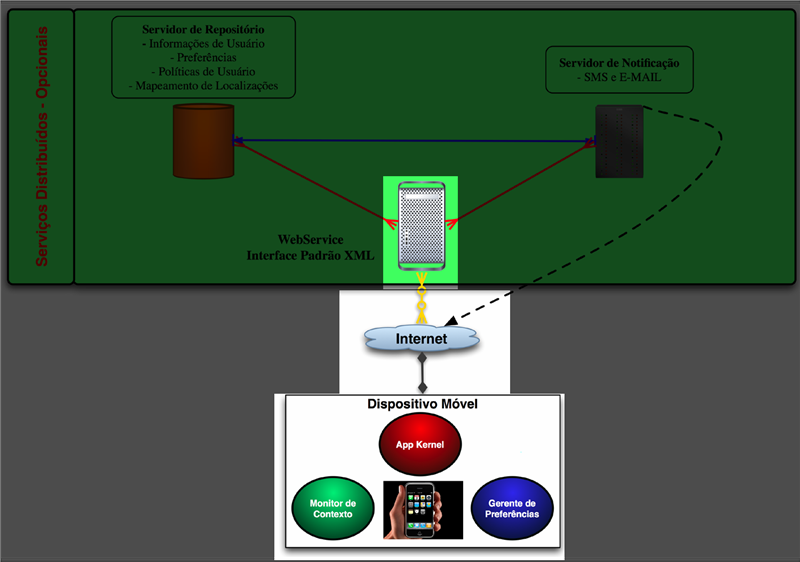
\includegraphics[width=0.80\textwidth]{../Pictures/Sequencias/Arquitetura_Distribuida/Conexao_Movel_WebService.png}
	\label{fig:ConexaoWebService}
\end{figure}

\end{frame}


\begin{frame}
  \frametitle{Arquitetura Distribu�da}
  \framesubtitle{Servidor de Reposit�rio}
  
\begin{figure}[htbp]
	\centering
		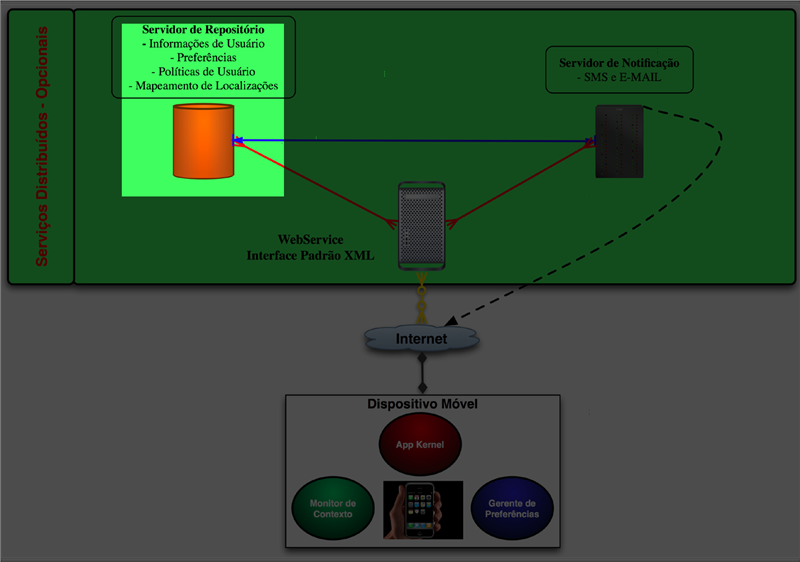
\includegraphics[width=0.80\textwidth]{../Pictures/Sequencias/Arquitetura_Distribuida/ServidorRepositorio.png}
	\label{fig:ServidorRepositorio}
\end{figure}

\end{frame}


\begin{frame}
  \frametitle{Arquitetura Distribu�da}
  \framesubtitle{Servidor de Notifica��es}
  
\begin{figure}[htbp]
	\centering
		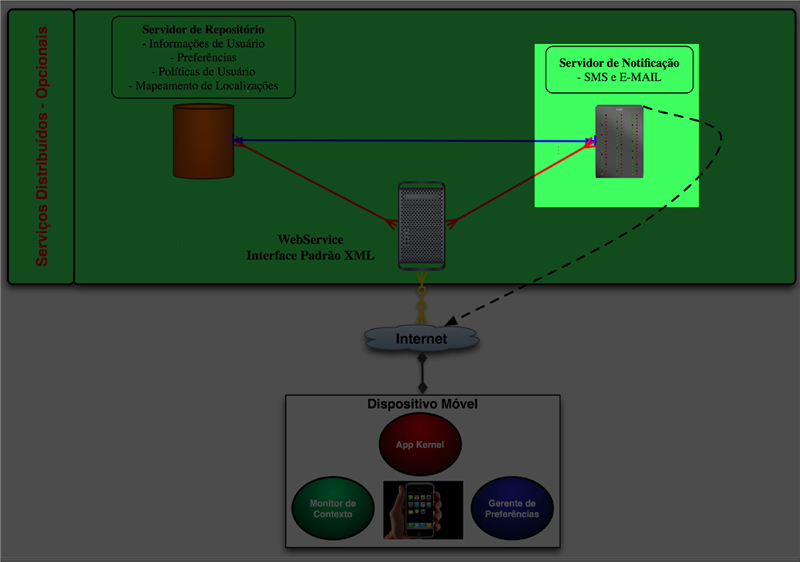
\includegraphics[width=0.80\textwidth]{../Pictures/Sequencias/Arquitetura_Distribuida/ServidorNotificacao.png}
	\label{fig:ServidorNotificacao}
\end{figure}

\end{frame}


\begin{frame}
  \frametitle{Arquitetura Distribu�da}
  \framesubtitle{Comunica��o \alert{entre os Servidores}}

\begin{figure}[htbp]
	\centering
		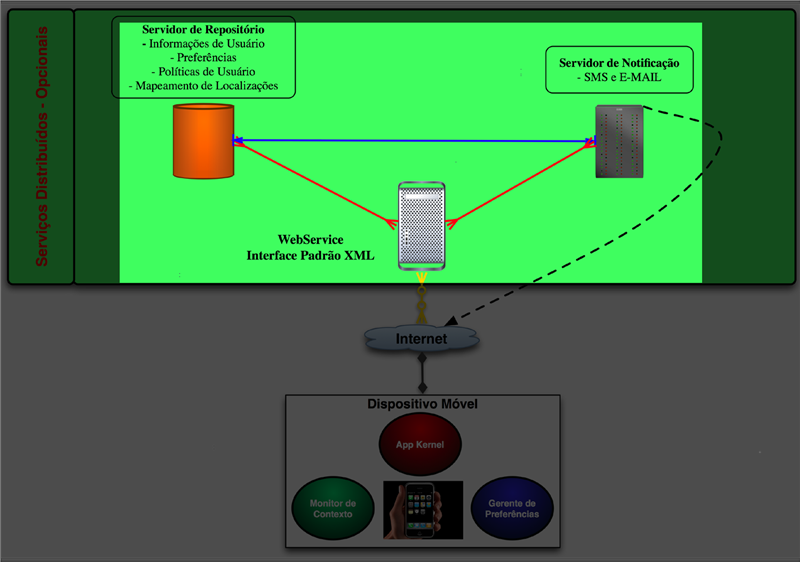
\includegraphics[width=0.80\textwidth]{../Pictures/Sequencias/Arquitetura_Distribuida/Conexao_Servidores.png}
	\label{fig:Conexao_Servidores}
\end{figure}

\end{frame}


\begin{frame}
  \frametitle{Arquitetura Distribu�da}
  \framesubtitle{Comunica��o entre \alert{Servidor WebService} e \alert{Servidor Reposit�rio}}
  
\begin{figure}[htbp]
	\centering
		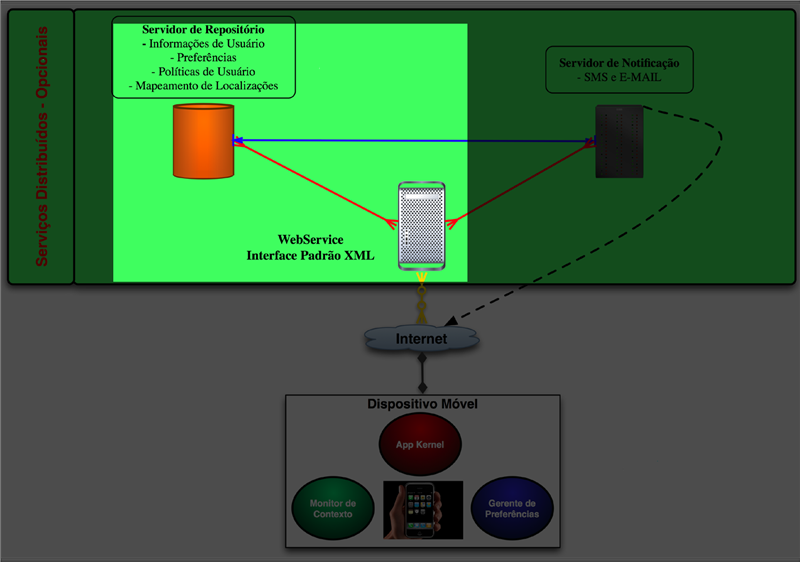
\includegraphics[width=0.80\textwidth]{../Pictures/Sequencias/Arquitetura_Distribuida/Conexao_WebService_BancoDados.png}
	\label{fig:Conexao_WebService_BancoDados}
\end{figure}

\end{frame}


\begin{frame}
  \frametitle{Arquitetura Distribu�da}
  \framesubtitle{Comunica��o entre \alert{Servidor WebService} e \alert{Servidor Notifica��o}}
  
\begin{figure}[htbp]
	\centering		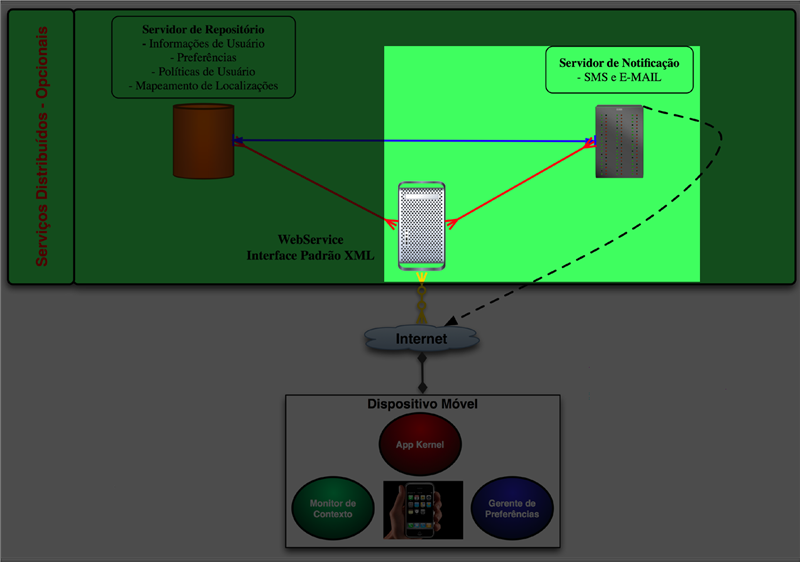
\includegraphics[width=0.80\textwidth]{../Pictures/Sequencias/Arquitetura_Distribuida/Conexao_WebService_Notificacao.png}
	\label{fig:Conexao_WebService_Notificacao}
\end{figure}

\end{frame}


\begin{frame}
  \frametitle{Arquitetura Distribu�da}
  \framesubtitle{Comunica��o entre \alert{Servidor Notifica��o} e \alert{Dispositivo M�vel}}
  
\begin{figure}[htbp]
	\centering
		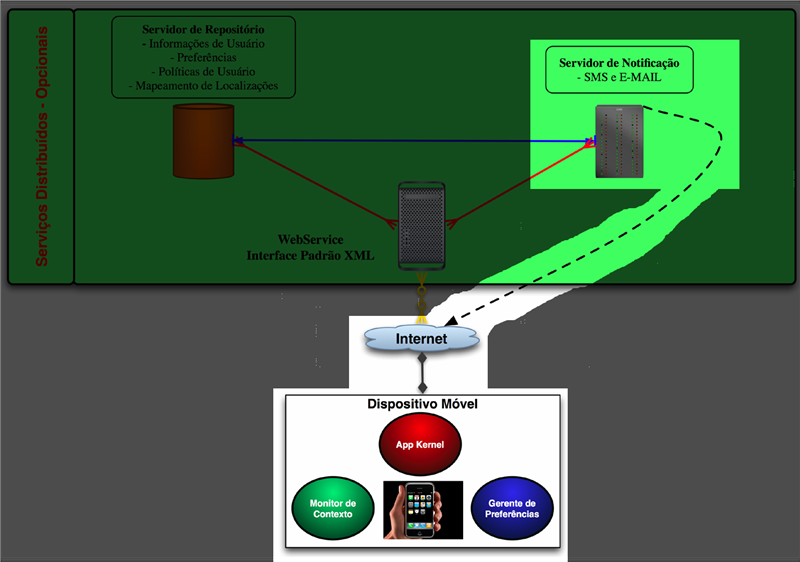
\includegraphics[width=0.80\textwidth]{../Pictures/Sequencias/Arquitetura_Distribuida/Conexao_Notificacao_Movel.png}
	\label{fig:Conexao_Notificacao_Movel}
\end{figure}

\end{frame}


\begin{frame}
  \frametitle{Arquitetura Distribu�da}
  \framesubtitle{Vis�o Geral}
  
\begin{figure}[htbp]
	\centering
		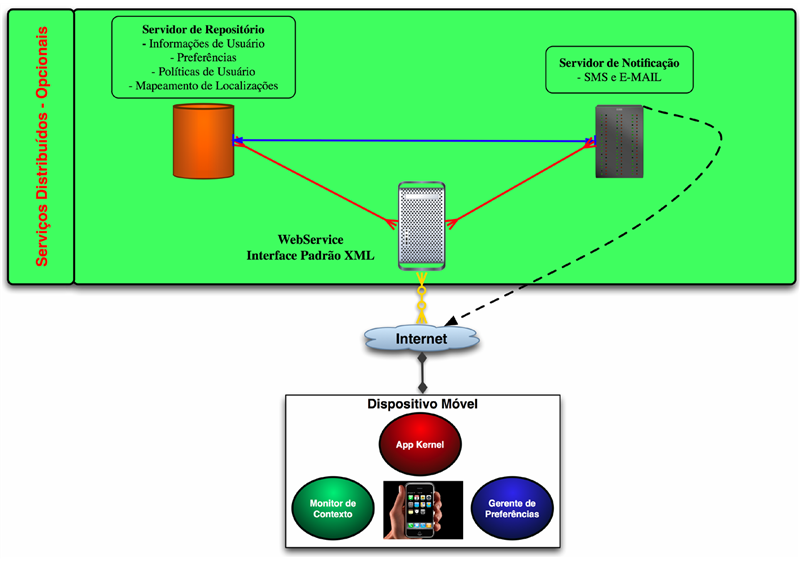
\includegraphics[width=0.80\textwidth]{../Pictures/Sequencias/Arquitetura_Distribuida/Arquitetura_Distribuida.png}
	\label{fig:Arquitetura_Distribuida}
\end{figure}

\end{frame}



%_______________________________________________________________________

\subsection{Pol�tica de Seguran�a Baseada em Localiza��o}

\begin{frame}
\frametitle{\alert{Pr�ximos Slides}}
  
  \textbf{Implementa��o da Pol�tica de Seguran�a Baseada em Localiza��o}.
	
	\beamerdefaultoverlayspecification{<+->}
	\begin{itemize}
		\item Identificar a Localiza��o do Usu�rio.
		\item Mapear �reas.
		\item Carregar Pol�ticas de Seguran�a Baseada na Localiza��o do Usu�rio.
	\end{itemize}
	\beamerdefaultoverlayspecification{<*>}
	
\end{frame}


\begin{frame}
		\begin{center}
			\huge \textbf{Identificar uma Localiza��o}.
		\end{center}
\end{frame}


\begin{frame}
  \frametitle{Identificar uma Localiza��o}
  \framesubtitle{Sele��o Manual}
  
				\begin{itemize}
						\item \textbf{Forma Padr�o:}
								\begin{enumerate}
									\item Selecionar manualmente a Localiza��o.
								\end{enumerate}
				\end{itemize}
								
				\begin{figure}[htbp]
						\centering
						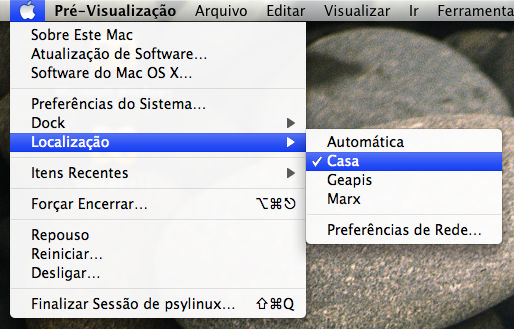
\includegraphics[width=0.60\textwidth]{../Pictures/Baixa/SelecaoManual.png}
						\label{fig:SelecaoManual}
				\end{figure}

\end{frame}


\begin{frame}
  \frametitle{Identificar uma Localiza��o}
  \framesubtitle{Sele��o Autom�tica \alert{(Opcional)}}								
			
	\begin{block}{Modos de Opera��o}
		\begin{enumerate}
				\item \alert{\textbf{Ambientes Outdoor:}}
						\begin{itemize}
								\item Usando o recurso \textbf{GPS} presente no dispositivo, caso exista.
						\end{itemize}	
		
				\item \alert{\textbf{Ambientes Indoor:}}
						\begin{itemize}
								\item Usando os recursos de \textbf{Localiza��o} oferecido pela \textbf{Arquitetura Distribu�da}.
						\end{itemize}
		\end{enumerate}
	\end{block}
								
\end{frame}


\begin{frame}
  \frametitle{\alert{GPS:} Identificar uma Localiza��o.}

			\begin{algorithm}[H]
				\SetLine	
				\textbf{Consulta} GPS \\
				$Local \longleftarrow raiz[ (x2{}-x1)\textsuperscript{\d 2} + (y2{}-y1)\textsuperscript{\d 2} ]$\;	
				\SetLine
				\Se	{$Local \subseteq banco.mapeamentos$}{
							\textbf{Selecione} $banco.mapeamento$\;
							\textbf{Carregue} $banco.politicas[Local]$\;
							\textbf{Carregue} $banco.preferencias[Local]$;				
				}
			\end{algorithm}

\end{frame}


\begin{frame}
\frametitle{\alert{Pr�ximos Slides}}

		\begin{center}
			\huge \textbf{Mapear uma �rea}.
		\end{center}
		
\end{frame}


\begin{frame}
  \frametitle{Mapear uma �rea (Introdu��o)}  
	
		\textbf{Discutiremos agora as abordagens de mapeamento relacionada aos t�picos abaixo:}
	
		\beamerdefaultoverlayspecification{<+->}
		\begin{itemize}
			\item Tipos de Mapeamento:
					\begin{enumerate}
						\item Indoor.
						\item Outdoor.
					\end{enumerate}
			\item O que � um mapeamento.
			\item Formas de mapeamento.
		\end{itemize}
		\beamerdefaultoverlayspecification{<*>} 
		 
\end{frame}


\begin{frame}
  \frametitle{Mapear uma �rea}
			
			\begin{itemize}
					\item Com a plataforma distribu�da o grupo \alert{Administrador} � capaz de mapear �reas comuns aos usu�rios.	
			\end{itemize}

			\begin{block}{Tipos de Mapeamento}					
					\begin{enumerate}
							\item As �reas comuns s�o definidas \textbf{exclusivamente} pelos administradores, e poder�o ser utilizadas por todos os usu�rios, \textit{ex.: Laborat�rio de Redes, Secretaria, Almoxarifado.}
				
							\item As �reas pessoais ser�o mapeadas pelo pr�prio usu�rio, e as mesmas n�o s�o vis�veis ou compartilhadas para os outros usu�rios  da plataforma.
					\end{enumerate}
  		\end{block}
\end{frame}


\begin{frame}
  \frametitle{Pol�tica de Seguran�a Baseada em Localiza��o}

  			\begin{figure}
					\centering
						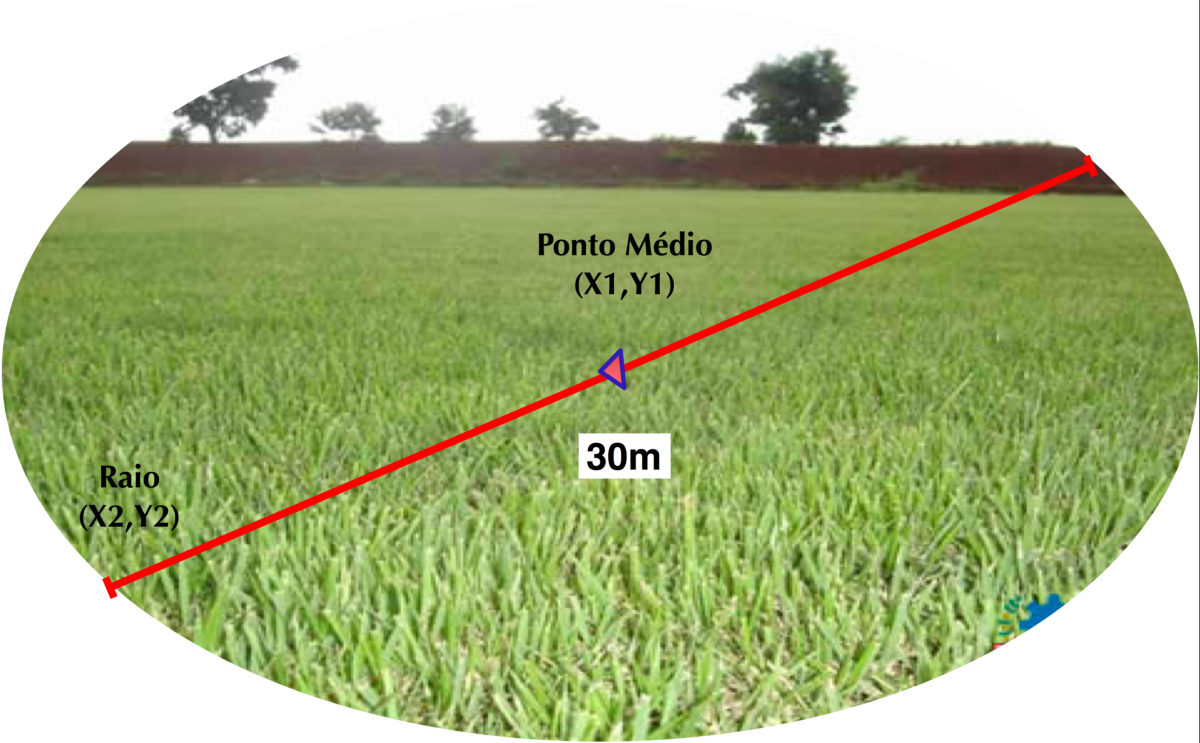
\includegraphics[width=0.90\textwidth]{../Pictures/Baixa/AlgoritmoGPS.png}
					\label{fig:AlgoritmoGPS}
				\end{figure}
				  
\end{frame}


\begin{frame}
  \frametitle{\alert{GPS:} Mapear uma �rea}

			\begin{algorithm}[H]
				\SetLine	
				\textbf{Consulta} GPS \\
				$Local \longleftarrow raiz[ (x2{}-x1)\textsuperscript{\d 2} + (y2{}-y1)\textsuperscript{\d 2} ]$\;	
				\SetLine
				\Se	{\textbf{n�o} ($Local \subseteq banco.mapeamentos$)}{			
						$distancia \longleftarrow raiz[(x1 {}- x2)2 + (y1 {}- y2)2]$\;
						$centro \longleftarrow distancia / 2$\;
						$area \longleftarrow 2 x Pi x (centro)2$\; 
						\textbf{Escreve} Entre com a Identifica��o para esta localiza��o\;
						\textbf{Salva} $Local$;
				}
			\end{algorithm}

\end{frame}

 
\begin{frame}
  \frametitle{Pol�tica de Seguran�a Baseada em Localiza��o}

   \begin{figure}[htb]
       \centering  % figura centralizada
       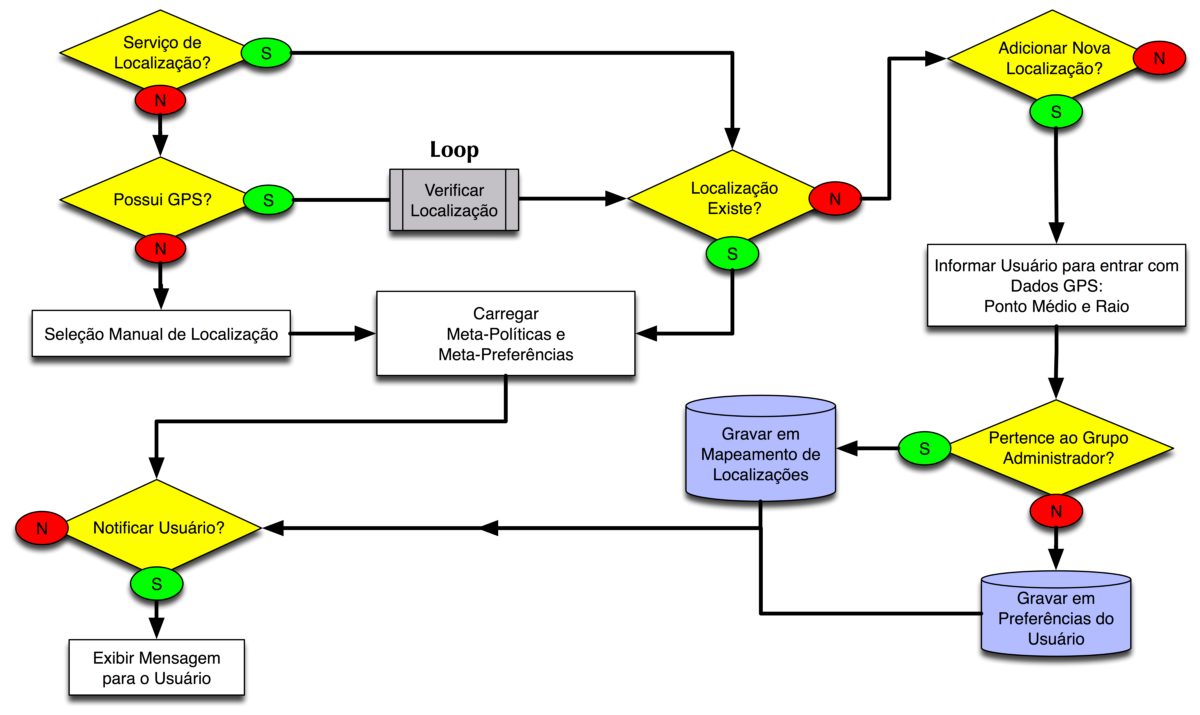
\includegraphics[width=0.90\textwidth]{../Pictures/Baixa/Fluxograma.png}
       \label{fig:Fluxograma}
   \end{figure}

\end{frame}


%_______________________________________________________________________

\subsection{Ilustrando o Funcionamento}

\begin{frame}
\frametitle{\alert{Pr�ximos Slides}}

		\begin{center}
			\huge \textbf{Ilustrando o Funcionamento}.
		\end{center}
		
\end{frame}


%%%%%%%%%%%%%%%%%%%%%%%%%%%%%%%%%%%%%%%%%%%%%%%%%%%%%%%%%%%%%%%%%%%%%%%%%%%%%%%%%%%%%%%
%% Cen�rio 1 - Carregando Meta-Pol�ticas e Meta-Prefer�ncias
%%%%%%%%%%%%%%%%%%%%%%%%%%%%%%%%%%%%%%%%%%%%%%%%%%%%%%%%%%%%%%%%%%%%%%%%%%%%%%%%%%%%%%%
\begin{frame}
  \frametitle{\textbf Dispositivo M�vel \alert{com} GPS}
  \framesubtitle{Carregando Meta-Pol�ticas e Meta-Prefer�ncias}

\begin{figure}[htbp]
	\centering
		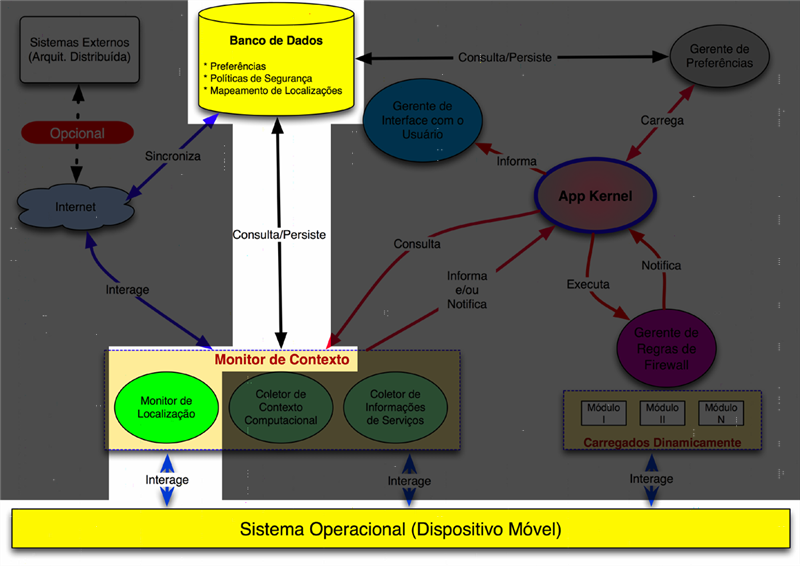
\includegraphics[width=0.80\textwidth]{../Pictures/Sequencias/Cenarios/CarregandoMetaDados_GPS/c1-1.png}
	\label{fig:c1-1}
\end{figure}

\end{frame}

\begin{frame}
  \frametitle{\textbf Dispositivo M�vel \alert{com} GPS}
  \framesubtitle{Carregando Meta-Pol�ticas e Meta-Prefer�ncias}

\begin{figure}[htbp]
	\centering
		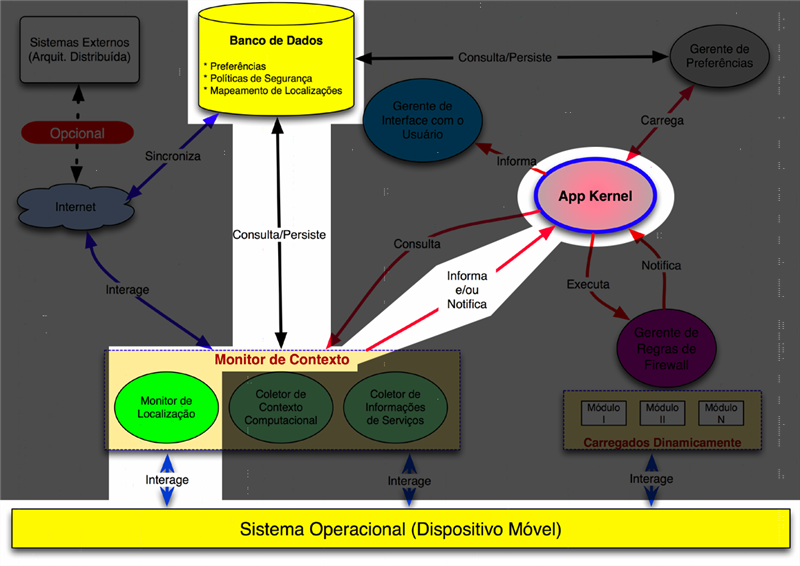
\includegraphics[width=0.80\textwidth]{../Pictures/Sequencias/Cenarios/CarregandoMetaDados_GPS/c1-2.png}
	\label{fig:c1-2}
\end{figure}

\end{frame}

\begin{frame}
\frametitle{\textbf Dispositivo M�vel \alert{com} GPS}
  \framesubtitle{Carregando Meta-Pol�ticas e Meta-Prefer�ncias}
  
\begin{figure}[htbp]
	\centering
		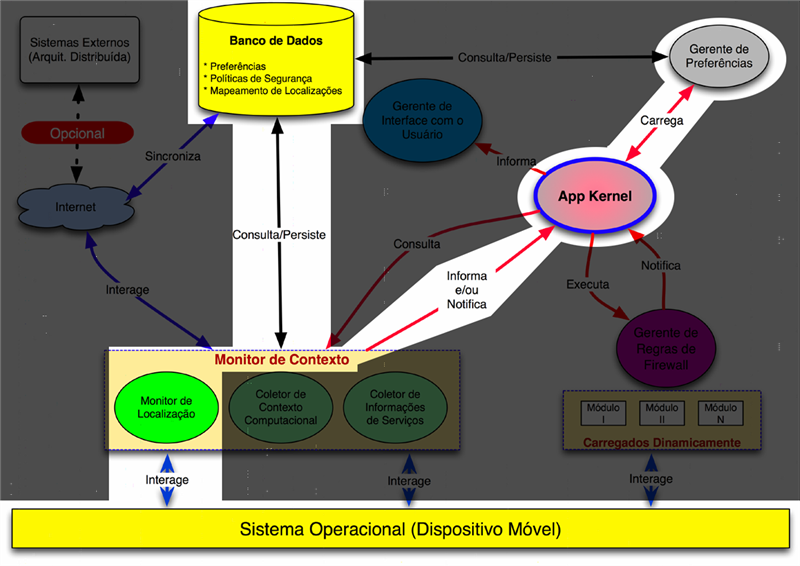
\includegraphics[width=0.80\textwidth]{../Pictures/Sequencias/Cenarios/CarregandoMetaDados_GPS/c1-3.png}
	\label{fig:c1-3}
\end{figure}

\end{frame}

\begin{frame}
  \frametitle{\textbf Dispositivo M�vel \alert{com} GPS}
  \framesubtitle{Carregando Meta-Pol�ticas e Meta-Prefer�ncias}

\begin{figure}[htbp]
	\centering
		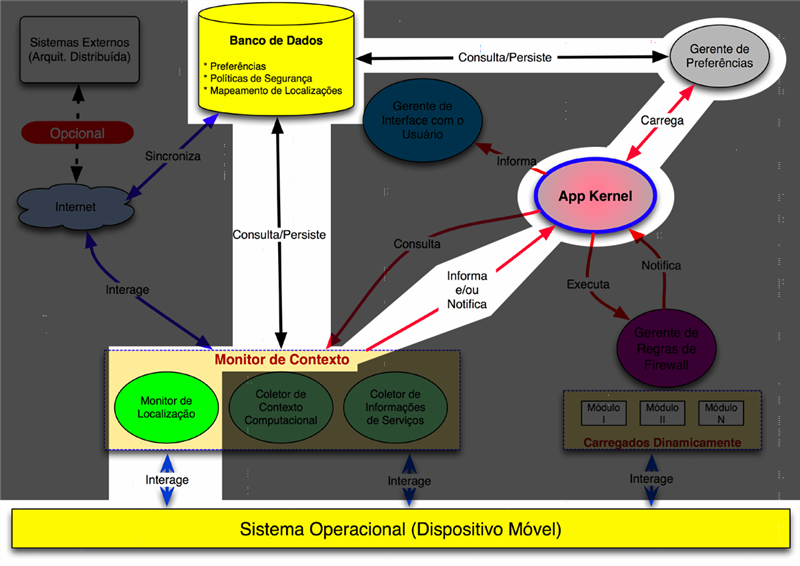
\includegraphics[width=0.80\textwidth]{../Pictures/Sequencias/Cenarios/CarregandoMetaDados_GPS/c1-4.png}
	\label{fig:c1-4}
\end{figure}

\end{frame}

\begin{frame}
  \frametitle{\textbf Dispositivo M�vel \alert{com} GPS}
  \framesubtitle{Carregando Meta-Pol�ticas e Meta-Prefer�ncias}

\begin{figure}[htbp]
	\centering
		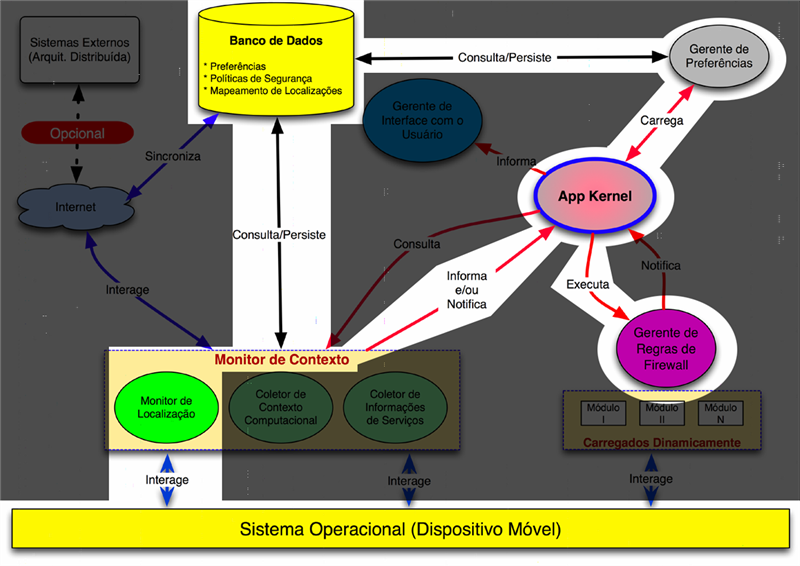
\includegraphics[width=0.80\textwidth]{../Pictures/Sequencias/Cenarios/CarregandoMetaDados_GPS/c1-5.png}
	\label{fig:c1-5}
\end{figure}

\end{frame}

\begin{frame}
  \frametitle{\textbf Dispositivo M�vel \alert{com} GPS}
  \framesubtitle{Carregando Meta-Pol�ticas e Meta-Prefer�ncias}

\begin{figure}[htbp]
	\centering
		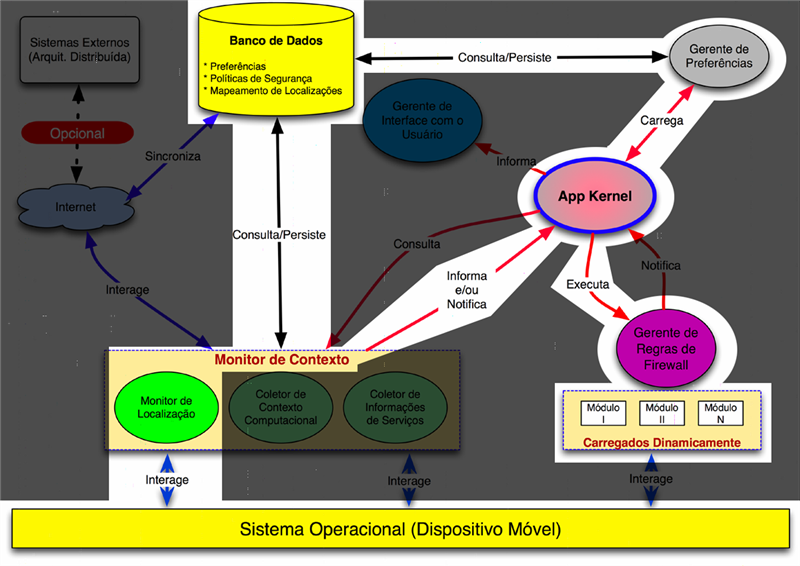
\includegraphics[width=0.80\textwidth]{../Pictures/Sequencias/Cenarios/CarregandoMetaDados_GPS/c1-6.png}
	\label{fig:c1-6}
\end{figure}

\end{frame}

\begin{frame}
  \frametitle{\textbf Dispositivo M�vel \alert{com} GPS}
  \framesubtitle{Carregando Meta-Pol�ticas e Meta-Prefer�ncias}

\begin{figure}[htbp]
	\centering
		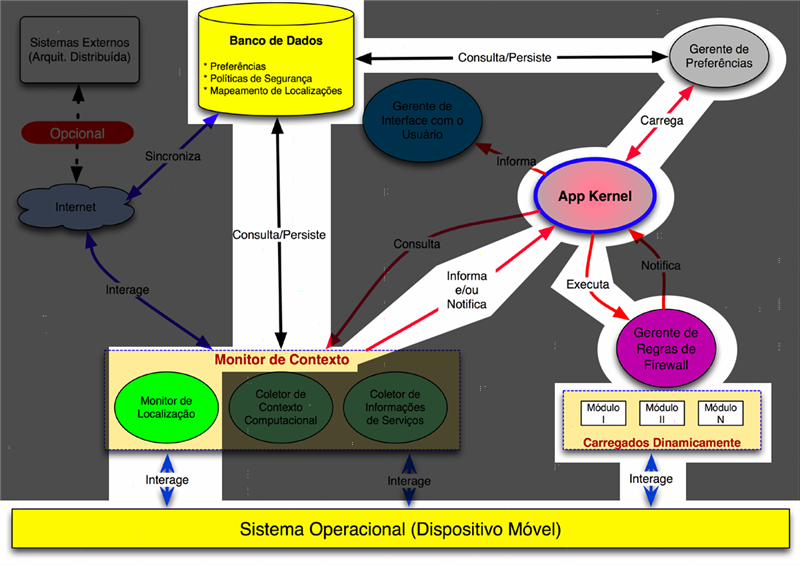
\includegraphics[width=0.80\textwidth]{../Pictures/Sequencias/Cenarios/CarregandoMetaDados_GPS/c1-7.png}
	\label{fig:c1-7}
\end{figure}

\end{frame}

\begin{frame}
  \frametitle{\textbf Dispositivo M�vel \alert{com} GPS}
  \framesubtitle{Carregando Meta-Pol�ticas e Meta-Prefer�ncias}

\begin{figure}[htbp]
	\centering
		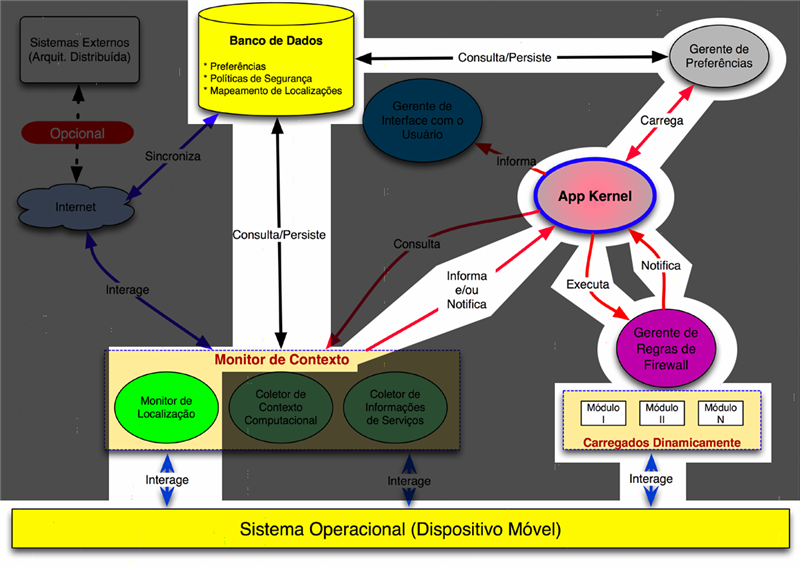
\includegraphics[width=0.80\textwidth]{../Pictures/Sequencias/Cenarios/CarregandoMetaDados_GPS/c1-8.png}
	\label{fig:c1-8}
\end{figure}

\end{frame}

\begin{frame}
  \frametitle{\textbf Dispositivo M�vel \alert{com} GPS}
  \framesubtitle{Carregando Meta-Pol�ticas e Meta-Prefer�ncias}

\begin{figure}[htbp]
	\centering
		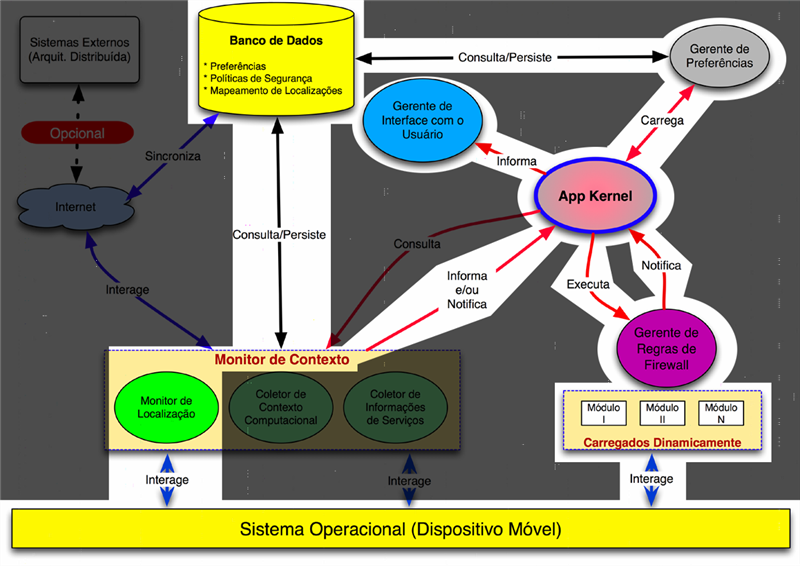
\includegraphics[width=0.80\textwidth]{../Pictures/Sequencias/Cenarios/CarregandoMetaDados_GPS/c1-9.png}
	\label{fig:c1-9}
\end{figure}

\end{frame}



%%%%%%%%%%%%%%%%%%%%%%%%%%%%%%%%%%%%%%%%%%%%%%%%%%%%%%%%%%%%%%%%%%%%%%%%%%%%%%%%%%%%%%%
%% Cen�rio 1 - Controlando Interfaces de Rede
%%%%%%%%%%%%%%%%%%%%%%%%%%%%%%%%%%%%%%%%%%%%%%%%%%%%%%%%%%%%%%%%%%%%%%%%%%%%%%%%%%%%%%%
\begin{frame}
  \frametitle{\textbf Controlando Interfaces de Rede}  

\begin{figure}[htbp]
	\centering
		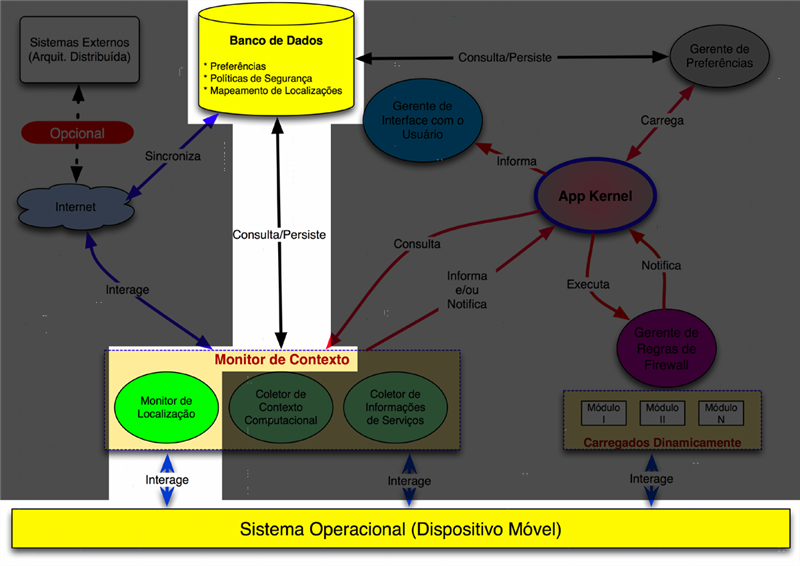
\includegraphics[width=0.80\textwidth]{../Pictures/Sequencias/Cenarios/ControlandoInterfaces/c2-1.png}
	\label{fig:c2-1}
\end{figure}

\end{frame}


\begin{frame}
  \frametitle{\textbf Controlando Interfaces de Rede}  

\begin{figure}[htbp]
	\centering
		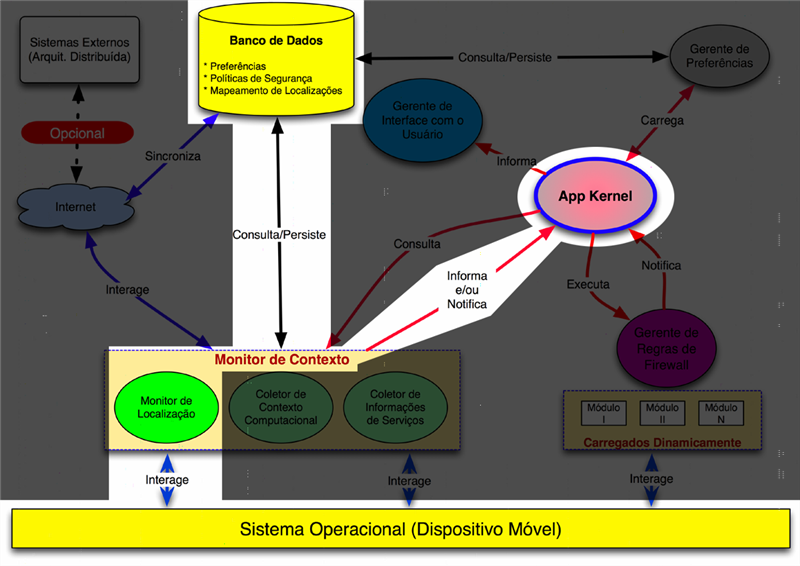
\includegraphics[width=0.80\textwidth]{../Pictures/Sequencias/Cenarios/ControlandoInterfaces/c2-2.png}
	\label{fig:c2-2}
\end{figure}

\end{frame}


\begin{frame}
  \frametitle{\textbf Controlando Interfaces de Rede}  

\begin{figure}[htbp]
	\centering
		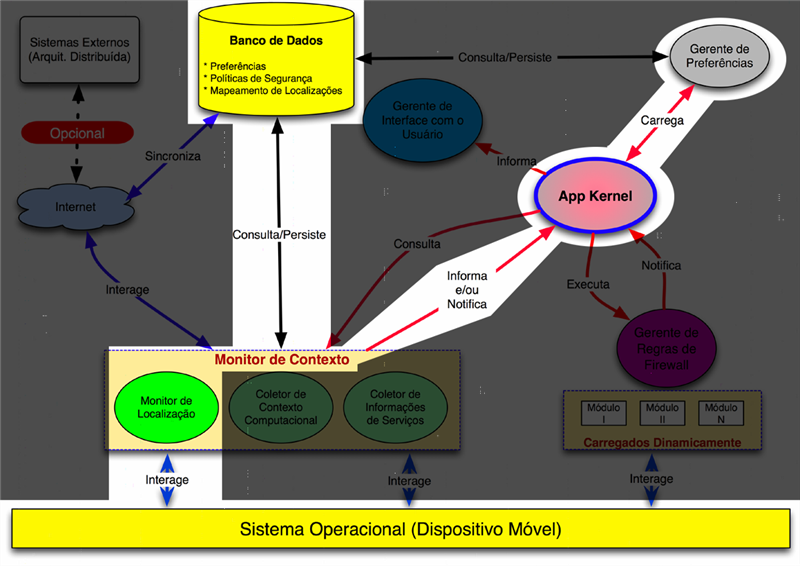
\includegraphics[width=0.80\textwidth]{../Pictures/Sequencias/Cenarios/ControlandoInterfaces/c2-3.png}
	\label{fig:c2-3}
\end{figure}

\end{frame}


\begin{frame}
  \frametitle{\textbf Controlando Interfaces de Rede}  

\begin{figure}[htbp]
	\centering
		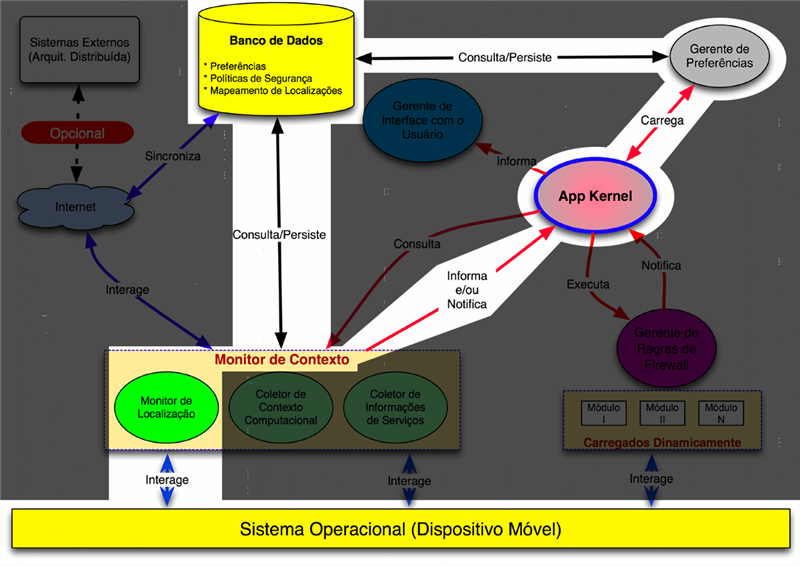
\includegraphics[width=0.80\textwidth]{../Pictures/Sequencias/Cenarios/ControlandoInterfaces/c2-4.png}
	\label{fig:c2-4}
\end{figure}

\end{frame}


\begin{frame}
  \frametitle{\textbf Controlando Interfaces de Rede}  

\begin{figure}[htbp]
	\centering
		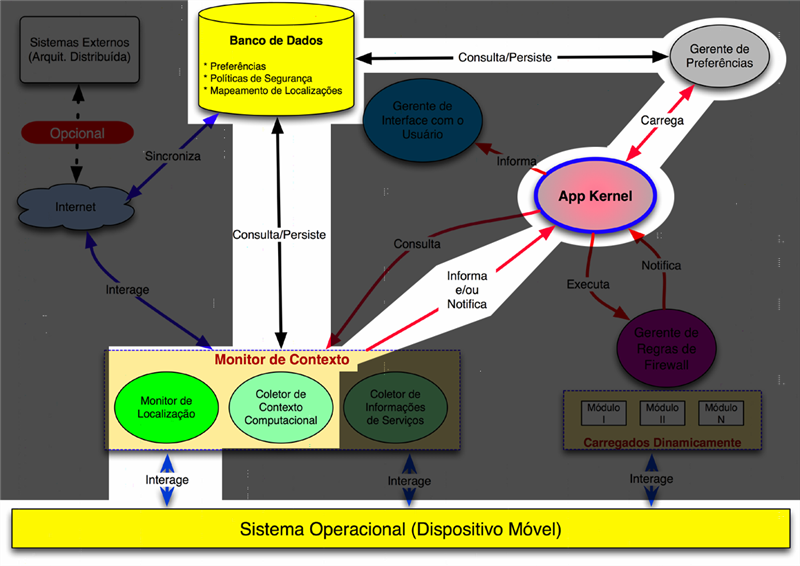
\includegraphics[width=0.80\textwidth]{../Pictures/Sequencias/Cenarios/ControlandoInterfaces/c2-5.png}
	\label{fig:c2-5}
\end{figure}

\end{frame}


\begin{frame}
  \frametitle{\textbf Controlando Interfaces de Rede}  

\begin{figure}[htbp]
	\centering
		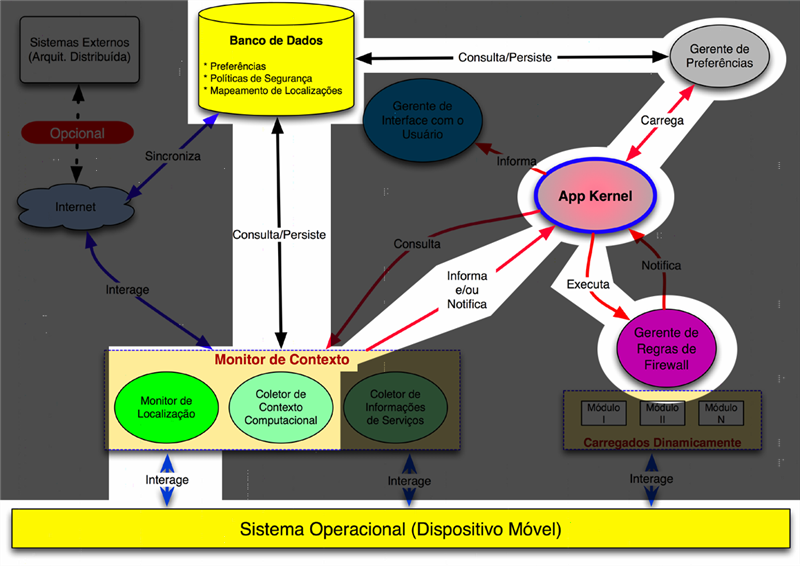
\includegraphics[width=0.80\textwidth]{../Pictures/Sequencias/Cenarios/ControlandoInterfaces/c2-6.png}
	\label{fig:c2-6}
\end{figure}

\end{frame}


\begin{frame}
  \frametitle{\textbf Controlando Interfaces de Rede}  

\begin{figure}[htbp]
	\centering
		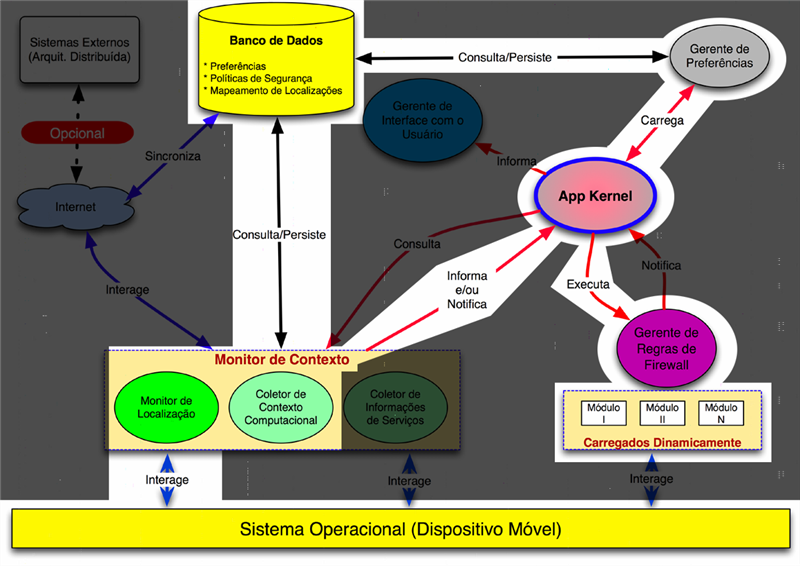
\includegraphics[width=0.80\textwidth]{../Pictures/Sequencias/Cenarios/ControlandoInterfaces/c2-7.png}
	\label{fig:c2-7}
\end{figure}

\end{frame}


\begin{frame}
  \frametitle{\textbf Controlando Interfaces de Rede}  

\begin{figure}[htbp]
	\centering
		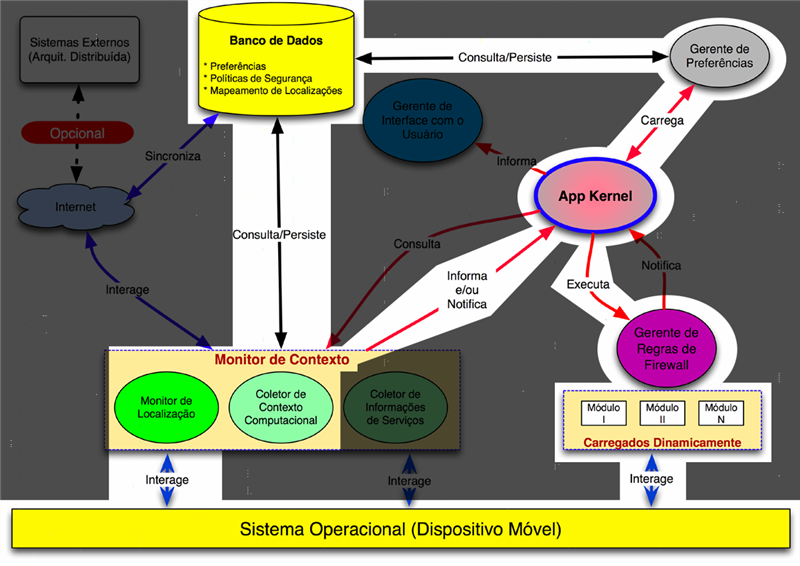
\includegraphics[width=0.80\textwidth]{../Pictures/Sequencias/Cenarios/ControlandoInterfaces/c2-8.png}
	\label{fig:c2-8}
\end{figure}

\end{frame}


\begin{frame}
  \frametitle{\textbf Controlando Interfaces de Rede}  

\begin{figure}[htbp]
	\centering
		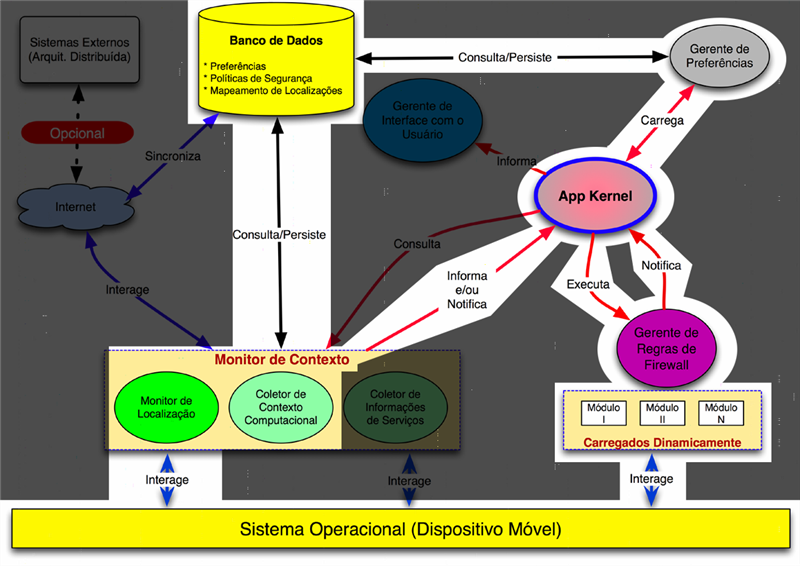
\includegraphics[width=0.80\textwidth]{../Pictures/Sequencias/Cenarios/ControlandoInterfaces/c2-9.png}
	\label{fig:c2-9}
\end{figure}

\end{frame}


\begin{frame}
  \frametitle{\textbf Controlando Interfaces de Rede}  

\begin{figure}[htbp]
	\centering
		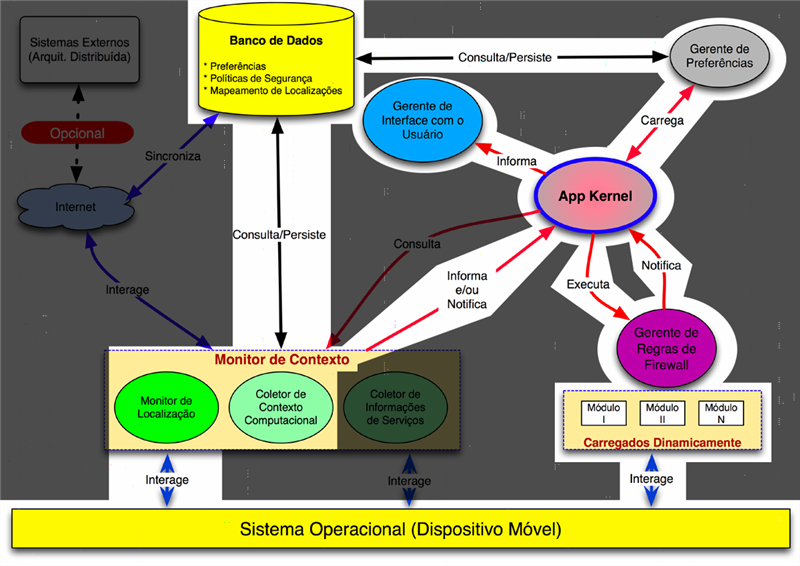
\includegraphics[width=0.80\textwidth]{../Pictures/Sequencias/Cenarios/ControlandoInterfaces/c2-10.png}
	\label{fig:c2-10}
\end{figure}

\end{frame}


%%%%%%%%%%%%%%%%%%%%%%%%%%%%%%%%%%%%%%%%%%%%%%%%%%%%%%%%%%%%%%%%%%%%%%%%%%%%%%%%%%%%%%%
%% Cen�rio 3 - Restringindo acessos entrantes e/ou saintes
%%%%%%%%%%%%%%%%%%%%%%%%%%%%%%%%%%%%%%%%%%%%%%%%%%%%%%%%%%%%%%%%%%%%%%%%%%%%%%%%%%%%%%%
\begin{frame}
  \frametitle{\textbf Restringindo acessos}  

\begin{figure}[htbp]
	\centering
		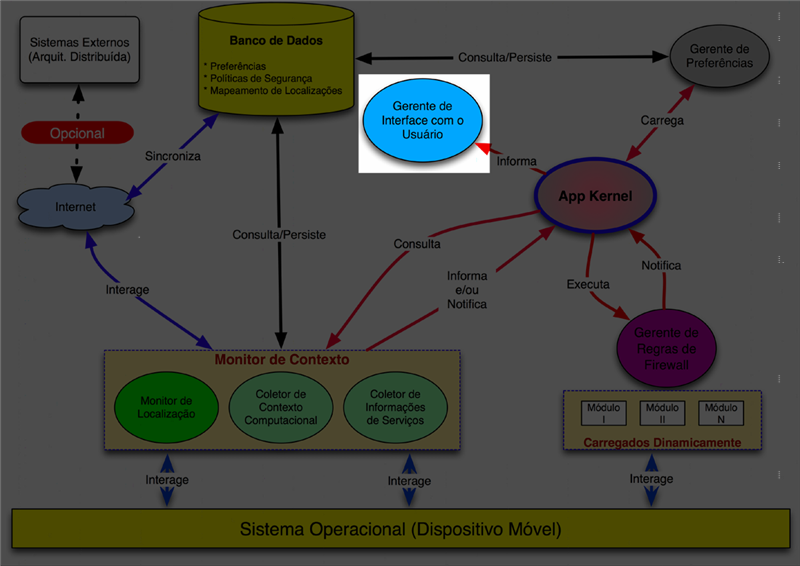
\includegraphics[width=0.80\textwidth]{../Pictures/Sequencias/Cenarios/ControlandoAcessos/c3-1.png}
	\label{fig:c3-1}
\end{figure}

\end{frame}


\begin{frame}
  \frametitle{\textbf Restringindo acessos}  

\begin{figure}[htbp]
	\centering
		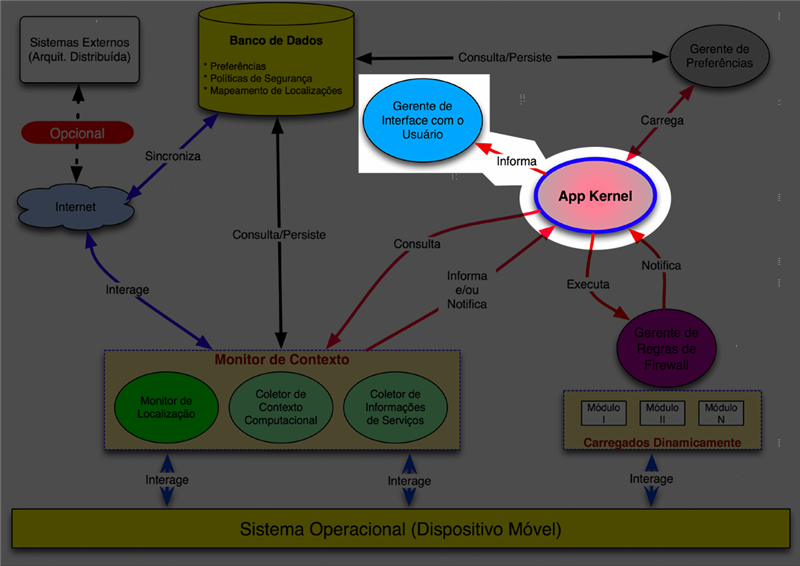
\includegraphics[width=0.80\textwidth]{../Pictures/Sequencias/Cenarios/ControlandoAcessos/c3-2.png}
	\label{fig:c3-2}
\end{figure}

\end{frame}


\begin{frame}
  \frametitle{\textbf Restringindo acessos}  

\begin{figure}[htbp]
	\centering
		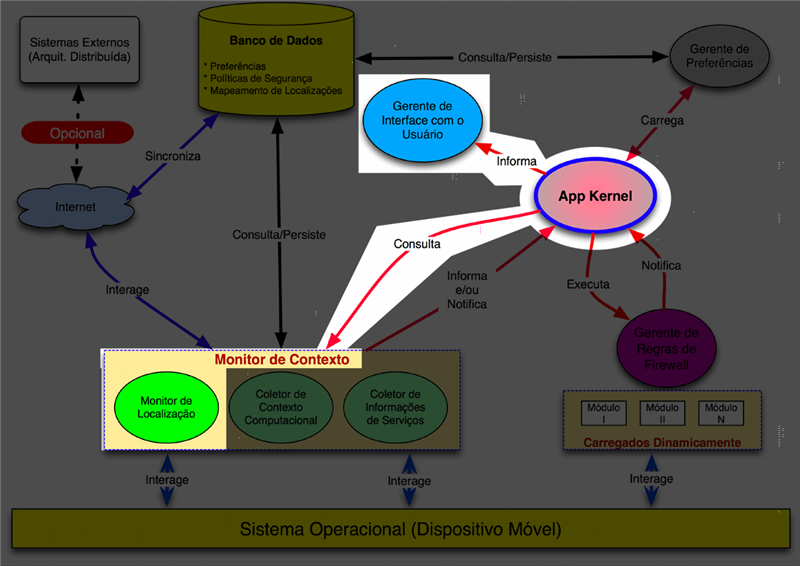
\includegraphics[width=0.80\textwidth]{../Pictures/Sequencias/Cenarios/ControlandoAcessos/c3-3.png}
	\label{fig:c3-3}
\end{figure}

\end{frame}


\begin{frame}
  \frametitle{\textbf Restringindo acessos}  

\begin{figure}[htbp]
	\centering
		\includegraphics[width=0.80\textwidth]{../Pictures/Sequencias/Cenarios/ControlandoAcessos/c3-4.png}
	\label{fig:c3-4}
\end{figure}

\end{frame}


\begin{frame}
  \frametitle{\textbf Restringindo acessos}  

\begin{figure}[htbp]
	\centering
		\includegraphics[width=0.80\textwidth]{../Pictures/Sequencias/Cenarios/ControlandoAcessos/c3-5.png}
	\label{fig:c3-5}
\end{figure}

\end{frame}


\begin{frame}
  \frametitle{\textbf Restringindo acessos}  

\begin{figure}[htbp]
	\centering
		\includegraphics[width=0.80\textwidth]{../Pictures/Sequencias/Cenarios/ControlandoAcessos/c3-6.png}
	\label{fig:c3-6}
\end{figure}

\end{frame}


\begin{frame}
  \frametitle{\textbf Restringindo acessos}  

\begin{figure}[htbp]
	\centering
		\includegraphics[width=0.80\textwidth]{../Pictures/Sequencias/Cenarios/ControlandoAcessos/c3-7.png}
	\label{fig:c3-7}
\end{figure}

\end{frame}


\begin{frame}
  \frametitle{\textbf Restringindo acessos}  

\begin{figure}[htbp]
	\centering
		\includegraphics[width=0.80\textwidth]{../Pictures/Sequencias/Cenarios/ControlandoAcessos/c3-8.png}
	\label{fig:c3-8}
\end{figure}

\end{frame}


\begin{frame}
  \frametitle{\textbf Restringindo acessos}  

\begin{figure}[htbp]
	\centering
		\includegraphics[width=0.80\textwidth]{../Pictures/Sequencias/Cenarios/ControlandoAcessos/c3-9.png}
	\label{fig:c3-9}
\end{figure}

\end{frame}


\begin{frame}
  \frametitle{\textbf Restringindo acessos}  

\begin{figure}[htbp]
	\centering
		\includegraphics[width=0.80\textwidth]{../Pictures/Sequencias/Cenarios/ControlandoAcessos/c3-10.png}
	\label{fig:c3-10}
\end{figure}

\end{frame}


\begin{frame}
  \frametitle{\textbf Restringindo acessos}  

\begin{figure}[htbp]
	\centering
		\includegraphics[width=0.80\textwidth]{../Pictures/Sequencias/Cenarios/ControlandoAcessos/c3-11.png}
	\label{fig:c3-11}
\end{figure}

\end{frame}


\begin{frame}
  \frametitle{\textbf Restringindo acessos}  

\begin{figure}[htbp]
	\centering
		\includegraphics[width=0.80\textwidth]{../Pictures/Sequencias/Cenarios/ControlandoAcessos/c3-12.png}
	\label{fig:c3-12}
\end{figure}

\end{frame}


%%%%%%%%%%%%%%%%%%%%%%%%%%%%%%%%%%%%%%%%%%%%%%%%%%%%%%%%%%%%%%%%%%%%%%%%%%%%%%%%%%%%%%%
%% Cen�rio 4 - Sincroniza��o Manual do Banco de Dados
%%%%%%%%%%%%%%%%%%%%%%%%%%%%%%%%%%%%%%%%%%%%%%%%%%%%%%%%%%%%%%%%%%%%%%%%%%%%%%%%%%%%%%%
\begin{frame}
  \frametitle{\textbf Sincroniza��o Manual do Banco de Dados}  

\begin{figure}[htbp]
	\centering
		\includegraphics[width=0.80\textwidth]{../Pictures/Sequencias/Cenarios/SincronizandoBancoManual/c4-1.png}
	\label{fig:c4-1}
\end{figure}

\end{frame}


\begin{frame}
  \frametitle{\textbf Sincroniza��o Manual do Banco de Dados}  

\begin{figure}[htbp]
	\centering
		\includegraphics[width=0.80\textwidth]{../Pictures/Sequencias/Cenarios/SincronizandoBancoManual/c4-2.png}
	\label{fig:c4-2}
\end{figure}

\end{frame}


\begin{frame}
  \frametitle{\textbf Sincroniza��o Manual do Banco de Dados}  

\begin{figure}[htbp]
	\centering
		\includegraphics[width=0.80\textwidth]{../Pictures/Sequencias/Cenarios/SincronizandoBancoManual/c4-3.png}
	\label{fig:c4-3}
\end{figure}

\end{frame}


\begin{frame}
  \frametitle{\textbf Sincroniza��o Manual do Banco de Dados}  

\begin{figure}[htbp]
	\centering
		\includegraphics[width=0.80\textwidth]{../Pictures/Sequencias/Cenarios/SincronizandoBancoManual/c4-4.png}
	\label{fig:c4-4}
\end{figure}

\end{frame}


\begin{frame}
  \frametitle{\textbf Sincroniza��o Manual do Banco de Dados}  

\begin{figure}[htbp]
	\centering
		\includegraphics[width=0.80\textwidth]{../Pictures/Sequencias/Cenarios/SincronizandoBancoManual/c4-5.png}
	\label{fig:c4-5}
\end{figure}

\end{frame}


\begin{frame}
  \frametitle{\textbf Sincroniza��o Manual do Banco de Dados}  

\begin{figure}[htbp]
	\centering
		\includegraphics[width=0.80\textwidth]{../Pictures/Sequencias/Cenarios/SincronizandoBancoManual/c4-6.png}
	\label{fig:c4-6}
\end{figure}

\end{frame}


\begin{frame}
  \frametitle{\textbf Sincroniza��o Manual do Banco de Dados}  

\begin{figure}[htbp]
	\centering
		\includegraphics[width=0.80\textwidth]{../Pictures/Sequencias/Cenarios/SincronizandoBancoManual/c4-7.png}
	\label{fig:c4-7}
\end{figure}

\end{frame}


\begin{frame}
  \frametitle{\textbf Sincroniza��o Manual do Banco de Dados}  

\begin{figure}[htbp]
	\centering
		\includegraphics[width=0.80\textwidth]{../Pictures/Sequencias/Cenarios/SincronizandoBancoManual/c4-8.png}
	\label{fig:c4-8}
\end{figure}

\end{frame}

\begin{frame}
  \frametitle{\textbf Sincroniza��o Manual do Banco de Dados}  

\begin{figure}[htbp]
	\centering
		\includegraphics[width=0.80\textwidth]{../Pictures/Sequencias/Cenarios/SincronizandoBancoManual/c4-9.png}
	\label{fig:c4-9}
\end{figure}

\end{frame}

